\part{Introduction}


\chapter{Histroy}

Style sheets have existed in one form or another since the beginnings of Standard Generalized Markup Language (SGML) in the 1980s. Cascading Style Sheets were developed as a means for creating a consistent approach to providing style information for web documents.


As HTML grew, it came to encompass a wider variety of stylistic capabilities to meet the demands of web developers. This evolution gave the designer more control over site appearance, at the cost of more complex HTML. Variations in web browser implementations, such as ViolaWWW and WorldWideWeb, made consistent site appearance difficult, and users had less control over how web content was displayed. Robert Cailliau wanted to separate the structure from the presentation. The ideal way would be to give the user different options and transferring three different kinds of style sheets: one for printing, one for the presentation on the screen and one for the editor feature.


To improve web presentation capabilities, nine different style sheet languages were proposed to the World Wide Web Consortium's (W3C) www-style mailing list. Of the nine proposals, two were chosen as the foundation for what became CSS: Cascading HTML Style Sheets (CHSS) and Stream-based Style Sheet Proposal (SSP). CHSS, a language that has some resemblance to today's CSS, was proposed by Håkon Wium Lie in October 1994. Bert Bos was working on a browser called Argo, which used its own style sheet language called SSP. Lie and Yves Lafon joined Dave Raggett to expand the Arena browser for supporting CSS as a testbed application for the W3C.[8][9][10] Lie and Bos worked together to develop the CSS standard (the 'H' was removed from the name because these style sheets could also be applied to other markup languages besides HTML).

Unlike existing style languages like DSSSL and FOSI, CSS allowed a document's style to be influenced by multiple style sheets. One style sheet could inherit or "cascade" from another, permitting a mixture of stylistic preferences controlled equally by the site designer and user.


Lie's proposal was presented at the "Mosaic and the Web" conference (later called WWW2) in Chicago, Illinois in 1994, and again with Bert Bos in 1995. Around this time the W3C was already being established, and took an interest in the development of CSS. It organized a workshop toward that end chaired by Steven Pemberton. This resulted in W3C adding work on CSS to the deliverables of the HTML editorial review board (ERB). Lie and Bos were the primary technical staff on this aspect of the project, with additional members, including Thomas Reardon of Microsoft, participating as well. In August 1996 Netscape Communication Corporation presented an alternative style sheet language called JavaScript Style Sheets (JSSS). The spec was never finished and is deprecated. By the end of 1996, CSS was ready to become official, and the CSS level 1 Recommendation was published in December.

Development of HTML, CSS, and the DOM had all been taking place in one group, the HTML Editorial Review Board (ERB). Early in 1997, the ERB was split into three working groups: HTML Working group, chaired by Dan Connolly of W3C; DOM Working group, chaired by Lauren Wood of SoftQuad; and CSS Working group, chaired by Chris Lilley of W3C.

The CSS Working Group began tackling issues that had not been addressed with CSS level 1, resulting in the creation of CSS level 2 on November 4, 1997. It was published as a W3C Recommendation on May 12, 1998. CSS level 3, which was started in 1998, is still under development as of 2009.

In 2005 the CSS Working Groups decided to enforce the requirements for standards more strictly. This meant that already published standards like CSS 2.1, CSS 3 Selectors and CSS 3 Text were pulled back from Candidate Recommendation to Working Draft level.

从1990年代初HTML被发明开始,样式表就以各种形式出现了,不同的浏览器结合了它们各自的样式语言,读者可以使用这些样式语言来调节网页的显示方式。一开始样式表是给读者用的,最初的HTML版本只含有很少的显示属性,读者来决定网页应该怎样被显示。

但随着HTML的成长,为了满足设计师的要求,HTML获得了很多显示功能。随着这些功能的增加外来定义样式的语言越来越没有意义了。

1994年哈坤·利提出了CSS的最初建议。伯特·波斯(Bert Bos)当时正在设计一个叫做“Argo”的浏览器,他们决定一起合作设计CSS。

当时已经有过一些样式表语言的建议了,但CSS是第一个含有“层叠”的主意的。在CSS中,一个文件的样式可以从其他的样式表中继承下来。读者在有些地方可以使用他自己更喜欢的样式,在其他地方则继承,或“层叠”作者的样式。这种层叠的方式使作者和读者都可以灵活地加入自己的设计,混合各人的爱好。

哈坤于1994年在芝加哥的一次会议上第一次展示了CSS的建议,1995年他与波斯一起再次展示这个建议。当时W3C刚刚创建,W3C对CSS的发展很感兴趣,它为此组织了一次讨论会。哈坤、波斯和其他一些人(比如微软的托马斯·雷尔登)是这个项目的主要技术负责人。1996年底,CSS已经完成。1996年12月CSS要求的第一版本被出版。

1997年初,W3C内组织了专门管CSS的工作组,其负责人是克里斯·里雷。这个工作组开始讨论第一版中没有涉及到的问题,其结果是1998年5月出版的第二版要求。到2007年为止,第三版还未完备。




\section{Difficulty with adoption}


The CSS 1 specification was completed in 1996. Microsoft's Internet Explorer 3 was released in that year, featuring some limited support for CSS. But it was more than three years before any web browser achieved near-full implementation of the specification. Internet Explorer 5.0 for the Macintosh, shipped in March 2000, was the first browser to have full (better than 99 percent) CSS 1 support, surpassing Opera, which had been the leader since its introduction of CSS support 15 months earlier. Other browsers followed soon afterwards, and many of them additionally implemented parts of CSS 2. As of August 2010, no (finished) browser had fully implemented CSS 2, with implementation levels varying.


Even though early browsers such as Internet Explorer 3[11] and 4, and Netscape 4.x had support for CSS, it was typically incomplete and had many bugs that prevented their implementations from being usefully adopted.


When later `version 5' browsers began to offer a fairly full implementation of CSS, they were still incorrect in certain areas and were fraught with inconsistencies, bugs and other quirks. The proliferation of such CSS-related inconsistencies and even the variation in feature support has made it difficult for designers to achieve a consistent appearance across browsers and platforms. Some authors resorted to workarounds such as CSS hacks and CSS filters.

Problems with browsers' patchy adoption of CSS, along with errata in the original specification, led the W3C to revise the CSS 2 standard into CSS 2.1, which moved nearer to a working snapshot of current CSS support in HTML browsers. Some CSS 2 properties that no browser successfully implemented were dropped, and in a few cases, defined behaviors were changed to bring the standard into line with the predominant existing implementations. CSS 2.1 became a Candidate Recommendation on February 25, 2004, but CSS 2.1 was pulled back to Working Draft status on June 13, 2005, and only returned to Candidate Recommendation status on July 19, 2007.


In the past, some web servers were configured to serve all documents with the filename extension .css as mime type application/x-pointplus rather than text/css. At the time, there was a software product on the market to convert PowerPoint files into Compact Slide Show files using the .css extension.



CSS最重要的目标是将文件的内容与它的显示分隔开来。在CSS出现前,几乎所有的HTML文件内都包含文件显示的信息,比如字体的颜色、背景应该是怎样的、如何排列、边缘、连线等等都必须一一在HTML文件内列出,有时重复列出。

CSS使作者可以将这些信息中的大部分隔离出来,简化HTML文件,这些信息被放在一个辅助的,用CSS语言写的文件中。HTML文件中只包含结构和内容的信息,CSS文件中只包含样式的信息。

比如HTML中H2标志这一个二级标题,它在级别上比一级标题H1低,比三级标题H3高。这些信息都是结构上的信息。一般来说级别越高的标题其字体也越大,H1的字体最大,因为一般来说字体越大它表示的内容就越重要,此外一般标题都使用粗体字,来突出它们的重要性。一般来说H2使用粗体字,其字体比H3大,比H1小,这些信息是显示用的信息。


在CSS出现前,假如作者要确定H2标题的颜色、字形、大小或其他显示特征的话,他要使用HTML中的font或其他样式指令,光H2不够,因为H2只是一个结构指令。假如一个标题要用斜体字、红色的字符、白色的底色的话,作者要这样写:

\begin{lstlisting}[language=HTML]
<H2><font color="red" bgcolor="white"><i>使用CSS</i></font></H2>
\end{lstlisting}

这些显示用的指令使得一个HTML变得非常复杂,要维护也比较困难。假如所有的二级标题都要这样来显示的话,所有的二级标题的指令都要这么复杂。此外,读者无法改变这些规定,假如一个读者更喜欢蓝色的标题的话,他无法改变标题的颜色,因为文件的作者特别规定了标题的颜色。

使用CSS的话H2指令只规定文章的结构,其显示由样式表来规定,上面的例子可以变成这样:


\begin{lstlisting}[language=HTML]
<H2>使用CSS</H2>
\end{lstlisting}

服从的样式表可以规定H2指令使用斜体字,红色字和白色背景:

\begin{lstlisting}[language=CSS]
H2 { 
    color: red; 
    background: white; 
    font-style: italic; 
}
\end{lstlisting}


这样显示与内容就分开了(由于CSS的优点,W3C现在正在考虑将HTML中的许多显示用的指令废弃掉)。HTML只表达文章的结构,CSS表达所有的显示。CSS可以指示颜色、字形、排列、大小以及其他许多非视觉的表达方式,比如将一篇文件的内容读出来。


CSS样式信息可以包含在一个附件中或包含在HTML文件内。读者可以使用多个样式表,在重复的情况下他可以选择其中之一,不同的媒体(media)可以使用不同的样式表。比如一个文件在荧光屏上的显示可以与在打印机中打印出来的显示不同,这样作者可以为不同的媒体设计最佳的显示方式。

此外CSS的目标之一是让读者有更大的控制显示的自由。假如一个读者觉得斜体字的标题读起来很困难,他可以使用自己的样式表文件,这个样式表可以“层叠”使用,他可以只改变红色斜体字这个样式而保留所有其他的样式。

\begin{lstlisting}[language=HTML]
<?xml version="1.0" encoding="utf-8"?>
<!DOCTYPE html PUBLIC "-//W3C//DTD XHTML 1.0 Strict//EN"
               "http://www.w3.org/TR/xhtml1/DTD/xhtml1-strict.dtd">
<html xmlns="http://www.w3.org/1999/xhtml" xml:lang="zh">
<head>
    <style type="text/css">
    body{
        background:#fff;
        color:#777;
    }
    h1{
        font:bold italic sans-serif;
        color:green;
    }
    </style>
</head>
<body>
    <h1>这个句子用綠色、粗体和斜体字显示</h1>
    <p>普通字。</p>
    <h1 style="color:red; background:green;">
    这个句子用大的、红色斜体字在绿色背景上显示,通用的h1样式在这里被取代了。
    </h1>
    <h1 style="color: green;"><strong><em>这个句子用綠色、粗体和斜体字显示</em></strong></h1>
</body>
</html>
\end{lstlisting}

浏览器可以自定义样式表,比如文件 highlightheaders.css 的内容可能是:

\begin{lstlisting}[language=CSS]
H1 {color: white; background: orange !important; }
H2 {color: white; background: green !important; }
\end{lstlisting}

这样的文件被贮存在访客的计算机内,他在浏览器内记录下显示时使用这个文件,其中\texttt{!important}表示在显示时使用读者的规定,而不是作者的规定。

有时一个网页的作者会滥用CSS。有些习惯于只使用HTML的作者可能会忽视CSS提供的可能性,比如有些习惯于使用HTML的显示元素的作者可能会在所有的HTML文件内加入CSS样式。这比将HTML显示和结构指令混在一起是一个进步,但它还是有许多同样的缺点,而且维护时的工作量与混合使用差不多。

CSS与其他编程语言有着一些共同的陷阱,尤其在命名CSS的 id 和 class 时。CSS作者常选择一个比较有说明性的名称而使用显示特征作为它们的名称,比如一个作者可能使用``big-red"来命名一个用大红字体的突出显示的字节。在当时,对作者来说这个名称可能是很直觉的,但假如后来作者决定突出显示的字节应该使用绿色,而不是红色的话,他的命名就有问题了。在上面这个例子中,一个更合适的名称应该是``emphasized"(强调),它描写的是这个``class"的用意,而不是它是如何被显示的。

另一个问题是未记录的、未定义的和往往会被遗忘的名称。一个网页作者可能会选择上百个名称,比如footer、footnote或者explanation、note、info、more可能是指同一回事。这样许多重复的名称就出现了,有时一个复杂的网站的设计者可能会结合HTML和CSS来解决这个问题,但这样一来他又把内容与显示黏有一起了,而且这样一来这个文件就只适合于某一媒体\footnote{外部样式表的一个大优点就是它是跨媒体的,因为不同的样式可以特别适用于不同的输出媒体。}了。


HTML本身的复杂性是另一个困难处。虽然大部分使用CSS的文件比传统的使用表格的文件要整洁,但过分使用class和过于细腻的结构层次同样使HTML变得繁庸。此外有的作者过分使用 div 元素。


另一个陷阱是为了解决常见的浏览器错误而引入特别的CSS样式,这些样式当然是为了除错而引入的,但它们使一个CSS文件的维护性能降低,有时这样的CSS文件的维护量甚至比过去的HTML文件的维护量还大。常见的特别CSS样式多是针对Internet Explorer (尤其IE 6、IE7 等旧版本)的显示错误而额外编写。

有时一个作者可能会过度地使用CSS来决定他的文件应该怎样被显示,例如一个作者会决定隐藏超链接底下的横线,这很容易做到,但对浏览者来说这可能会带来不便。


有些新的CSS3 样式尚未成为标准,因此在使用时需要加上前缀(Prefix)\footnote{从Internet Explorer 10 Release Preview 起, transform、transition、animation和gradient渐变等属性均可不加前缀。},使其可以在采用不同排版引擎的浏览器中正确显示,例如使用transition 时,需要额外撰写四行编码:


\begin{lstlisting}[language=CSS]
-webkit-transition: height 0.2s linear; /* 针对使用WebKit排版引擎的浏览器,如Google Chrome、Apple Safari */
-moz-transition: height 0.2s linear; /* 针对使用Gecko排版引擎的浏览器,如Mozilla Firefox */
-o-transition: height 0.2s linear; /* 针对使用Presto排版引擎的浏览器,如Opera */
-ms-transition: height 0.2s linear; /* MSIE, 但 Release Preview 起可以不用前缀 */
transition: height 0.2s linear; /* CSS3标准,放最后 */
\end{lstlisting}

CSS 的文件大小因此增大,到这些 CSS 样式不需要前缀时,又需要额外花时间把它们删除。




\section{Variations}


CSS has various levels and profiles. Each level of CSS builds upon the last, typically adding new features and typically denoted as CSS 1, CSS 2, CSS 3, and CSS 4. Profiles are typically a subset of one or more levels of CSS built for a particular device or user interface. Currently there are profiles for mobile devices, printers, and television sets. Profiles should not be confused with media types, which were added in CSS 2.




\subsection{CSS 1}

The first CSS specification to become an official W3C Recommendation is CSS level 1, published in December 1996. Among its capabilities are support for

\begin{compactitem}
\item  Font properties such as typeface and emphasis
\item Color of text, backgrounds, and other elements
\item Text attributes such as spacing between words, letters, and lines of text
\item Alignment of text, images, tables and other elements
\item Margin, border, padding, and positioning for most elements
\item Unique identification and generic classification of groups of attributes
\end{compactitem}

The W3C no longer maintains the CSS 1 Recommendation.

1994年,哈坤·利和伯特·波斯合作设计CSS。他们在1994年首次在芝加哥的一次会议上第一次展示了CSS的建议。1996年12月发表的CSS1的要求有(W3C管理CSS1要求):

\begin{compactitem}
\item 支持字体的大小、字形、强调
\item 支持字的颜色、背景的颜色和其他元素
\item 支持文章特征如字母、词和行之间的距离
\item 支持文字的排列、图像、表格和其他元素
\item 支持边缘、围框和其他关于排版的元素
\item 支持id和class
\end{compactitem}




\subsection{CSS 2}


CSS level 2 specification was developed by the W3C and published as a recommendation in May 1998. A superset of CSS 1, CSS 2 includes a number of new capabilities like absolute, relative, and fixed positioning of elements and z-index, the concept of media types, support for aural style sheets and bidirectional text, and new font properties such as shadows.

The W3C no longer maintains the CSS 2 recommendation.

1998年5月W3C发表了CSS2(W3C管理CSS2要求),其中包括新的内容如:

\begin{compactitem}
\item 绝对的、相对的和固定的定比特素、媒体型的概念、
\item 双向文件和一个新的字体。
\end{compactitem}

\subsection{CSS 2.1}


CSS level 2 revision 1, often referred to as "CSS 2.1", fixes errors in CSS 2, removes poorly supported or not fully interoperable features and adds already-implemented browser extensions to the specification. In order to comply with the W3C Process for standardizing technical specifications, CSS 2.1 went back and forth between Working Draft status and Candidate Recommendation status for many years. CSS 2.1 first became a Candidate Recommendation on February 25, 2004, but it was reverted to a Working Draft on June 13, 2005 for further review. It returned to Candidate Recommendation on 19 July 2007 and then updated twice in 2009. However, since changes and clarifications were made, it again went back to Last Call Working Draft on 7 December 2010.

CSS 2.1 went to Proposed Recommendation on 12 April 2011. After being reviewed by the W3C Advisory Committee, it was finally published as a W3C Recommendation on 7 June 2011.


CSS2.1修改了CSS2中的一些错误,删除了其中基本不被支持的内容和增加了一些已有的浏览器的扩展内容。


\subsection{CSS 3}

Unlike CSS 2, which is a large single specification defining various features, CSS 3 is divided into several separate documents called "modules". Each module adds new capabilities or extends features defined in CSS 2, preserving backward compatibility. Work on CSS level 3 started around the time of publication of the original CSS 2 recommendation. The earliest CSS 3 drafts were published in June 1999.


Due to the modularization, different modules have different stability and statuses. As of June 2012, there are over fifty CSS modules published from the CSS Working Group., and four of these have been published as formal recommendations:

\begin{compactitem}
\item 2012-06-19 : Media Queries
\item 2011-09-29 : Namespaces
\item 2011-09-29 : Selectors Level 3
\item 2011-06-07 : Color
\end{compactitem}

Some modules (including Backgrounds and Borders and Multi-column Layout among others) have Candidate Recommendation (CR) status and are considered moderately stable. At CR stage, implementations are advised to drop vendor prefixes.

CSS3 分成了不同类型,称为“modules”。而每一个“modules”都有于 CSS2 中额外增加的功能,以及向后兼容。

CSS3 早于1999年已开始制订,直到2011年6月7日, CSS 3 Color Module 终于发布为 W3C Recommendation。CSS3 里增加了不少功能,包括“border-radius”、“text-shadow”、“transform”以及“transition”等。


\begin{lstlisting}[language=CSS]
div{
    border-radius:10px;
    text-shadow:0px 2px 2px #AAA;
    box-shadow:0px 3px 10px #AAA;
    transform:rotate(-15deg);
}
\end{lstlisting}

把 <div> 圆角半径10像素(px),反时针旋转15度,加上2像素(px)的文字阴影,并加上10像素(px)的灰色阴影。


但由于现时不同浏览器仍需要加上不同的前缀,部分属性在Firefox需要加上\texttt{-moz-}、Safari以及Google Chrome需加上\texttt{-webkit-}、Opera需加上\texttt{-o-}、Internet Explorer 9里部份需加上\texttt{-ms-},所以需要写成这样︰

\begin{lstlisting}[language=CSS]
div{
    -webkit-border-radius:10px;
    -moz-border-radius:10px;
    border-radius:10px;
 
    text-shadow:0px 2px 2px #AAA;
 
    -webkit-box-shadow:0px 3px 10px #AAA;
    -moz-box-shadow:0px 3px 10px #AAA;
    box-shadow:0px 3px 10px #AAA;
 
    -webkit-transform:rotate(-15deg);
    -moz-transform:rotate(-15deg);
    -ms-transform:rotate(-15deg);
    -o-transform:rotate(-15deg);
    transform:rotate(-15deg);
}
\end{lstlisting}

CSS3 亦支持动画(animation)及立体(preserved-3d),但是只有内有 Webkit 的浏览器如 Safari 及 Google Chrome,基于 Trident 的 Internet Explorer 10,和基于 Gecko 的 Firefox (10 及以上版本)等浏览器支持。



\subsection{CSS 4}

There is no single, integrated CSS4 specification, since it is split into separate modules. However, there are ``level 4" modules.

Since CSS3 split the CSS language's definition into modules, the modules have been allowed to level independently. Most modules are level 3 - they build on things from CSS 2.1. A few level 4 modules exist (such as Image Values, Backgrounds \& Borders, or Selectors), which build on the functionality of a preceding level 3 module. Others define entirely new functionality, such as Flexbox.

So, while there is no monolithic ``CSS4" that will be worked on after ``CSS3" is finished completely, the level 4 modules can collectively be referred to as ``CSS4".

W3C于2011年9月29日开始了设计CSS4,直至现时只有极少数的功能被部分网页浏览器支持,如使用在HTML而非SVG上的pointer-events。


CSS4增加了一些更方便的方法以选择不同元素︰

\begin{compactitem}
\item 选择目标

\begin{lstlisting}[language=CSS]
$ul li.clicked {
    background: white;
}
\end{lstlisting}

CSS4里其中一项新功能就是能够定义于Selection Chain里哪一个是目标。于上例里,ul前面加了一个\$号,代表它就是要改变的目标,即“把里面有li(class是clicked)的ul的底色转为白色。”






\item \texttt{:matches()}


\begin{lstlisting}[language=CSS]
:matches(div, p, nav) span{
  font-size: 18px;
}
\end{lstlisting}

CSS4里其中另一项新功能就是能够是用\texttt{:matches()}来简化选择器,上方的例子等如︰

\begin{lstlisting}[language=CSS]
div span, p span, nav span{
  font-size: 18px;
}
\end{lstlisting}

事实上现在已有浏览器支持类似的功能,如Firefox和Webkit︰


\begin{lstlisting}[language=CSS]
/*Firefox使用-moz-前綴*/
-moz-any(div, p, nav) span{
  font-size: 18px;
}
/*Webkit使用-webkit-前綴*/
-webkit-any(div, p, nav) span{
  font-size: 18px;
}
\end{lstlisting}


\end{compactitem}



\section{Browser support}

Because not all browsers correctly parse CSS code, developed coding techniques known as CSS hacks can either filter specific browsers or target specific browsers (generally both are known as CSS filters). The former can be defined as CSS filtering hacks and the latter can be defined as CSS targeting hacks. Both can be used to hide or show parts of the CSS to different browsers. This is achieved either by exploiting CSS-handling quirks or bugs in the browser, or by taking advantage of lack of support for parts of the CSS specifications. Using CSS filters, some designers have gone as far as delivering different CSS to certain browsers to ensure designs render as expected. Because very early web browsers were either completely incapable of handling CSS, or rendered CSS very poorly, designers today often routinely use CSS filters that completely prevent these browsers from accessing any of the CSS. Internet Explorer support for CSS began with IE 3.0 and increased progressively with each version. By 2008, the first Beta of Internet Explorer 8 offered support for CSS 2.1 in its best web standards mode.

An example of a historically well-known CSS browser bug was the Internet Explorer box model bug, where box widths are interpreted incorrectly in several versions of the browser, resulting in blocks that are too narrow when viewed in Internet Explorer, but correct in standards-compliant browsers. The bug can be avoided in Internet Explorer 6 by using the correct doctype in (X)HTML documents. CSS hacks and CSS filters are used to compensate for bugs such as this, just one of hundreds of CSS bugs that have been documented in various versions of Netscape, Mozilla Firefox, Opera, and Internet Explorer (including Internet Explorer 7).


Even when the availability of CSS-capable browsers made CSS a viable technology, the adoption of CSS was still held back by designers' struggles with browsers' incorrect CSS implementation and patchy CSS support. Even today, these problems continue to make the business of CSS design more complex and costly than it was intended to be, and cross-browser testing remains a necessity. Other reasons for the continuing non-adoption of CSS are: its perceived complexity, authors' lack of familiarity with CSS syntax and required techniques, poor support from authoring tools, the risks posed by inconsistency between browsers and the increased costs of testing.

Currently there is strong competition between the WebKit layout engine used in Apple Safari and Google Chrome, the similar KHTML engine used in KDE's Konqueror browser and Mozilla's Gecko layout engine used in Firefox — each of them is leading in different aspects of CSS. As of August 2009, Internet Explorer 8, Firefox 2 and 3 have reasonably complete levels of implementation of CSS 2.1.

CSS信息可以来自:

\begin{compactitem}
\item 作者样式
	\begin{compactitem}
	\item 作者可以在他的HTML文件中确定一个外来的、独立的CSS文件(外部样式表),其优先级最低
	\item 作者可以将CSS信息包含在HTML文件内(内部样式表)
	\item 作者可以在一个HTML指令内结合CSS指令(内联样式),其优先级最高。一般这样做是为了在特殊情况下,把上面来源的CSS抵消掉
	\end{compactitem}	
\item 自定样式
	\begin{compactitem}
	\item 读者可以在他的浏览器内设立一个CSS文件。这个CSS文件可以用在所有的HTML文件上。假如作者的CSS文件与读者的相冲突,那么读者可以选择一个
	\end{compactitem}
\item 浏览器样式
	\begin{compactitem}
	\item 假如外部没有特别指定一个样式的话,一般浏览器自己有一个内在的样式
	\end{compactitem}
\end{compactitem}


尽管CSS1规格1996年就完成了,但一直到三年后还没有一个浏览器彻底实现了这些规格。2000年3月出版的微软在麦金塔电脑上运行的Internet Explorer 5.0是第一个彻底贯彻CSS1的浏览器。此后许多其他浏览器也贯彻了CSS1和CSS2的一部分。但到2004年为止还没有一个浏览器彻底贯彻了CSS2。尤其 aural 和 paged 等特性是被支持得最差的。

即使彻底贯彻了CSS1的浏览器也遇到了许多困难。许多CSS的贯彻互相矛盾、有错或有其他稀奇古怪的地方。为了使他们的页面在所有的浏览器中、在所有的系统上的显示相同,作者往往要使用特别的技巧或解决特殊的困难。

一个最著名的错误涉及到显示方形的宽度,在Internet Explorer浏览器中方形的宽度的显示有错误,其结果是方形的宽度在许多浏览器中被正确地显示,但在Internet Explorer上方形的宽度太窄。虽然这个错误有解决的办法,但它限制了其他一些功能(Internet Explorer 8.0已改善方形宽度显示问题)。


\section{Advantages}

\begin{compactitem}
\item \textbf{Separation of content from presentation}

CSS facilitates publication of content in multiple presentation formats based on nominal parameters. Nominal parameters include explicit user preferences, different web browsers, the type of device being used to view the content (a desktop computer or mobile Internet device), the geographic location of the user and many other variables.


\item \textbf{Site-wide consistency}

When CSS is used effectively, in terms of inheritance and ``cascading," a global style sheet can be used to affect and style elements site-wide. If the situation arises that the styling of the elements should need to be changed or adjusted, these changes can be made by editing rules in the global style sheet. Before CSS, this sort of maintenance was more difficult, expensive and time-consuming.

\item \textbf{Bandwidth}

A stylesheet, internal or external, will specify the style once for a range of HTML elements selected by class, type or relationship to others. This is much more efficient than repeating style information inline for each occurrence of the element. An external stylesheet is usually stored in the browser cache, and can therefore be used on multiple pages without being reloaded, further reducing data transfer over a network.

\item \textbf{Page reformatting}

With a simple change of one line, a different style sheet can be used for the same page. This has advantages for accessibility, as well as providing the ability to tailor a page or site to different target devices. Furthermore, devices not able to understand the styling still display the content.

\item \textbf{Accessibility}

Without CSS, web designers must typically lay out their pages with techniques such as HTML tables that hinder accessibility for vision-impaired users.+
\end{compactitem}



总结起来,网页的读者和作者都可以使用CSS来决定文件的颜色、字体、排版等显示特性,而CSS最主要的目的是将文件的内容与显示分隔开来,这有许多好处:

\begin{compactitem}
\item 文件的可读性加强
\item 文件的结构更加灵活
\item 作者和读者可以自己决定文件的显示
\item 文件的结构简化了
\end{compactitem}

CSS的具体优点包括如下几个方面:

\begin{compactitem}
\item 通过单个样式表控制多个文档的布局;
\item 更精确的布局控制;
\item 为不同的媒体类型(屏幕、打印等)采取不同的布局。
\end{compactitem}

另外,在HTML中:

\begin{compactitem}
\item 一个整个网站或其中一部分网页的显示信息被集中在一个地方,要改变它们很方便
\item 不同的读者可以有不同的样式,比如有的读者需要字体比较大
\item HTML文件本身的范围变小了,它的结构简单了,它不需要包含显示的信息
\end{compactitem}

CSS还可以控制其他参数,例如声音(假如浏览器有阅读功能的话)或给视觉障碍者用的感受装置。



\section{Limitations}


Some noted limitations of the current capabilities of CSS include:

\begin{compactitem}
\item \textbf{Selectors are unable to ascend}

CSS currently offers no way to select a parent or ancestor of an element that satisfies certain criteria. CSS Selectors Level 4, which is still in Working Draft status, proposes such a selector, but only as part of the ``complete" selector profile, not the ``fast" profile used in dynamic CSS styling. A more advanced selector scheme (such as XPath) would enable more sophisticated style sheets. The major reasons for the CSS Working Group previously rejecting proposals for parent selectors are related to browser performance and incremental rendering issues.

\item \textbf{Vertical control limitations}

While horizontal placement of elements is generally easy to control, vertical placement is frequently unintuitive, convoluted, or outright impossible. Simple tasks, such as centering an element vertically or getting a footer to be placed no higher than bottom of viewport, either require complicated and unintuitive style rules, or simple but widely unsupported rules.

\item \textbf{Absence of expressions}

There is currently no ability to specify property values as simple expressions (such as margin-left: 10\% – 3em + 4px;). This would be useful in a variety of cases, such as calculating the size of columns subject to a constraint on the sum of all columns. However, a working draft with a calc() value to address this limitation has been published by the CSS WG. Internet Explorer versions 5 to 7 support a proprietary expression() statement, with similar functionality. This proprietary expression() statement is no longer supported from Internet Explorer 8 onwards, except in compatibility modes. This decision was taken for "standards compliance, browser performance, and security reasons".

\item \textbf{Lack of column declaration}

While possible in current CSS 3 (using the column-count module), layouts with multiple columns can be complex to implement in CSS 2.1. With CSS 2.1, the process is often done using floating elements, which are often rendered differently by different browsers, different computer screen shapes, and different screen ratios set on standard monitors.

\item \textbf{Cannot explicitly declare new scope independently of position}

Scoping rules for properties such as z-index look for the closest parent element with a position:absolute or position:relative attribute. This odd coupling has undesired effects. For example, it is impossible to avoid declaring a new scope when one is forced to adjust an element's position, preventing one from using the desired scope of a parent element.

\item \textbf{Pseudo-class dynamic behavior not controllable}

CSS implements pseudo-classes that allow a degree of user feedback by conditional application of alternate styles. One CSS pseudo-class, ``:hover", is dynamic (equivalent of JavaScript ``onmouseover") and has potential for abuse (e.g., implementing cursor-proximity popups),[40] but CSS has no ability for a client to disable it (no ``disable"-like property) or limit its effects (no ``nochange"-like values for each property).

\item \textbf{Cannot name rules}

There is no way to name a CSS rule, which would allow (for example) client-side scripts to refer to the rule even if its selector changes.

\item \textbf{Cannot include styles from a rule into another rule}

CSS styles often must be duplicated in several rules to achieve a desired effect, causing additional maintenance and requiring more thorough testing.

\item \textbf{Cannot target specific text without altering markup}

Besides the :first-letter pseudo-element, one cannot target specific ranges of text without needing to utilize place-holder elements.
\end{compactitem}


CSS明显的缺点包括:

\begin{compactitem}
\item 浏览器不同的支持
\end{compactitem}

浏览器对CSS的支持没有统一,造成不同的浏览器显示效果不同。在微软Internet Explorer 的旧版本6.0中有许多独有的CSS 2.0属性,但错误显示很多重要的属性,例如:width,height,和float。

许多CSS编写人员为了尽可能在常用的各个浏览器中达到一致的版面编排,要写很多针对各个浏览器的不同的CSS代码。当版面编排很复杂时,要在各个浏览器里取得相同效果是不可能的。

\begin{compactitem}
\item CSS没有父选择器
\end{compactitem}

CSS选择器无法提供元素的继承性。先进的选择器(例如XPath)有助于复杂的样式设计。然而,浏览器的性能和增加彩现的问题,关系着父层选择器,却是CSS的工作组拒绝建议的主要原因,而CSS4则计划包括类似功能。

\begin{compactitem}
\item 不能明确地指定继承性
\end{compactitem}

样式的继承性,创建在浏览器中DOM元素的层级和具体的规则上,引用CSS2说明中的章节6.4.1 - \href{http://www.w3.org/TR/CSS2/cascade.html\#cascading-order}{Assigning property values, Cascading, and Inheritance}。

\begin{compactitem}
\item 垂直控制的局限
\end{compactitem}

元素的水平放置普遍地易于控制,垂直控制则不然。简单来说,垂直地围绕一个元素、页脚的放置不能高于可见视窗(viewport,视窗或屏幕的可见范围)的底部范围,这需要复杂的样式规则,或是规则简单,但不被广泛支持。

\begin{compactitem}
\item 没有算术功能
\end{compactitem}

直至 CSS 2.1 的CSS没有办法明确简单地进行计算(例如:\texttt{margin-left: 10\% - 3em + 4px;})。

计算功能在很多情况下都是非常有用的,例如总字段中计算字段的尺寸限制。无论如何,CSS WG发表了CSS局限性的草案。IE 5至IE 7提供\texttt{expression()}函数(即所谓的CSS表达式)来执行计算功能,例如\texttt{left: expression(document.body.offsetWidth - 110 + "px");} 。

为了与CSS标准看齐,并且\texttt{expression()}函数性能差,微软从IE 8开始停止支持此函数。但 CSS 3 中具有\texttt{calc()}表达式以执行计算功能,例如:

\begin{lstlisting}[language=CSS]
p {
    margin: calc(1rem - 2px) calc(1rem - 1px) 
}
\end{lstlisting}

\begin{compactitem}
\item 缺乏唯一性
\end{compactitem}

同样的效果可以用不同的属性来完成,这对不少的CSS编写人员造成困扰。例如position、display与float定义了不同的配置方式,而且不能有效的交替使用。

一个\texttt{display: table-cell}元素不能指定\texttt{float}或是\texttt{position: relative},因为指定\texttt{float: left}的元素不应该受到display效果的影响。

再者,没有考虑到新创建属性所造成的影响,例如在表格中应该使用\texttt{border-spacing}而不是\texttt{margin-*}来指定表格元素。这是因为依照CSS准则,表格内部元素是没有边界(margin)的。






\chapter{Syntax}

\vspace{-30pt}

\section{Style \& Content}




Cascading Style Sheets (CSS)\cite{css} is a style sheet language used for describing the presentation semantics (the look and formatting) of a document written in a markup language. Its most common application is to style web pages written in HTML and XHTML, but the language can also be applied to any kind of XML document, including plain XML, SVG and XUL.

CSS is designed primarily to enable the separation of document content (written in HTML or a similar markup language) from document presentation, including elements such as the layout, colors, and fonts. This separation can improve content accessibility, provide more flexibility and control in the specification of presentation characteristics, enable multiple pages to share formatting, and reduce complexity and repetition in the structural content (such as by allowing for tableless web design). CSS can also allow the same markup page to be presented in different styles for different rendering methods, such as on-screen, in print, by voice (when read out by a speech-based browser or screen reader) and on Braille-based, tactile devices. It can also be used to allow the web page to display differently depending on the screen size or device on which it is being viewed. While the author of a document typically links that document to a CSS file, readers can use a different style sheet, perhaps one on their own computer, to override the one the author has specified.

CSS specifies a priority scheme to determine which style rules apply if more than one rule matches against a particular element. In this so-called cascade, priorities or weights are calculated and assigned to rules, so that the results are predictable.

The CSS specifications are maintained by the World Wide Web Consortium (W3C). Internet media type (MIME type) text/css is registered for use with CSS by RFC 2318 (March 1998), and they also operate a free CSS validation service.

CSS has a simple syntax and uses a number of English keywords to specify the names of various style properties.

A style sheet consists of a list of rules. Each rule or rule-set consists of one or more selectors, and a declaration block.

Prior to CSS, nearly all of the presentational attributes of HTML documents were contained within the HTML markup; all font colors, background styles, element alignments, borders and sizes had to be explicitly described, often repeatedly, within the HTML. CSS allows authors to move much of that information to another file, the style sheet, resulting in considerably simpler HTML.


Headings (h1 elements), sub-headings (h2), sub-sub-headings (h3), etc., are defined structurally using HTML. In print and on the screen, choice of font, size, color and emphasis for these elements is presentational.



在Tim Berners-Lee发明万维网(World Wide Web)时,HTML语言是唯一用于给文本添加结构的语言。

HTML标签原本被设计为用于定义文档内容,开发者可以通过使用类似<h1>、<p>这样的标签来表达“这是一个标题”(利用h1标签)或“这是一个段落”(利用p标签)的目的,同时文档布局由浏览器来完成,不使用任何的格式化标签。


随着Web逐渐流行起来,网页设计者们开始寻求为网页增添布局的可能性。为此,当时的浏览器厂商们(网景公司和微软公司)发明了一些新的HTML标签(比如<font>等)来引入新的布局——而非新的结构,这导致了原本用于文本结构化的标签(比如<table>等)越来越多地被误用于进行页面的布局。许多新的布局标签(比如<blink>)往往只有一种浏览器支持。

由于当时两种主要的浏览器(Netscape 和 Internet Explorer)不断地将新的 HTML 标签和属性(比如字体标签和颜色属性)添加到HTML实现中,导致想要创建文档内容清晰地独立于文档表现层的站点变得越来越困难。



为了解决这个问题,非营利的标准化联盟W3C(万维网联盟)肩负起了 HTML 标准化的使命,并在 HTML 4.0 之外创造出样式(Style)。现在所有的主流浏览器均支持层叠样式表,从而使Web设计师们拥有了完善的、所有浏览器都支持的布局能力,而且表现样式与内容的分离,也令网站维护容易了许多。





以前,使用HTML在为网站添加布局效果的同时,也存在被误用的可能。作为一种样式表语言,CSS可以定义如何显示HTML元素,包括字体、颜色、边距、高度、宽度、背景图像、高级定位等方面。相比之下,CSS提供了更多选择,而且更为精确、完善,因而可以这样说,HTML用于结构化内容,CSS用于格式化结构化的内容。

\section{Basics}

层叠样式表(Cascading Style Sheets,简写CSS),又称串样式列表、层次结构式样式表文件,一种用来为结构化文档(如HTML文档或XML应用)添加样式(字体、间距和颜色等)的计算机语言,由W3C定义和维护\footnote{目前最新版本是CSS2.1,为W3C的推荐标准,CSS3现在已被大部分现代浏览器支持,而下一版的CSS4仍在开发过程中。}。





CSS由多组“规则”组成。每个规则由两个主要的部分构成:选择器(selector),以及一条或多条声明。

\begin{lstlisting}[language=CSS]
selector {
    declaration1;
    declaration2; 
    ... 
    declarationN
}
\end{lstlisting}

选择器通常是开发者需要改变样式的 HTML 元素,而每条声明由一个属性(property)和一个值(value)组成,属性和值之间用半角冒号(:)隔开,属性和值合称为“特性”。多个特性间用“;”隔开,最后用“\texttt{\{ \}}”括起来。


\begin{lstlisting}[language=CSS]
selector {
    property: value;
}
\end{lstlisting}

\begin{compactitem}
\item 选择器(Selector):多个选择器可以半角逗号(,)隔开。
\item 属性(property):CSS1、CSS2、CSS3规定了许多的属性,目的在控制选择器的样式。
\item 值(value):指属性接受的设置值,多个关键字时大都以空格隔开。
\end{compactitem}


许多CSS属性都与HTML属性相似,如下所示:

\begin{figure}[!h]
\centering
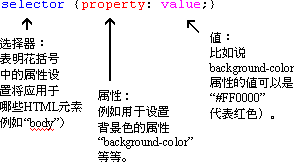
\includegraphics[scale=0.6]{css_attribute_structure.pdf}
\vspace{-10pt}

\caption{基本的CSS模型}
\label{css_attribute_structure}
\end{figure}

下面这行代码的作用是将 h1 元素内的文字颜色定义为红色,同时将字体大小设置为 14 像素。在这个例子中,h1 是选择器,color 和 font-size 是属性,red 和 14px 是值。

\begin{lstlisting}[language=CSS]
h1 { color:red; font-size:14px; }
\end{lstlisting}

下面的示意图为我们展示了上面这段代码的结构:

\begin{figure}[!h]
\centering
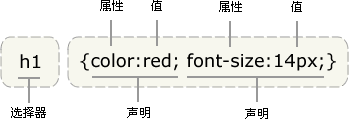
\includegraphics[scale=0.5]{css_selector.png}
\vspace{-10pt}
\caption{CSS 选择器}
\label{css_selector}
\end{figure}

其中,属性是开发者希望设置的样式属性(style attribute),每个属性有一个值,属性和值被冒号分开。

如果要定义不止一个声明,则需要用分号将每个声明分开。下面的例子展示出如何定义一个红色文字的居中段落,就像这样:

\begin{lstlisting}[language=CSS]
p {
    font-family: "sans serif"; 
    text-align: center; 
    color:red;
}
\end{lstlisting}

一般情况下,应该在每行只描述一个属性,这样可以增强样式定义的可读性。如果值为若干单词,则要给值加引号。

最后一条声明是不需要加分号的,因为分号在英语中是一个分隔符号,不是结束符号。然而,大多数有经验的设计师会在每条声明的末尾都加上分号,这么做的好处是,当从现有的规则中增减声明时,会尽可能地减少出错的可能性。

是否包含空格不会影响 CSS 在浏览器的工作效果,同样,与XHTML不同,CSS对大小写不敏感。不过存在一个例外,如果涉及到与 HTML 文档一起工作的话,\texttt{class}和\texttt{id}名称对大小写是敏感的。

大多数样式表包含不止一条规则,而大多数规则包含不止一个声明。多重声明和空格的使用使得样式表更容易被编辑:

\begin{lstlisting}[language=CSS]
body {
  color: #000;
  background: #fff;
  margin: 0;
  padding: 0;
  font-family: Georgia, Palatino, serif, "sans serif";
}
\end{lstlisting}




对于颜色,除了英文单词 red,还可以使用十六进制的颜色值~\#ff0000:

\begin{lstlisting}[language=CSS]
h1 {
    color: #ff0000; 
    font-size: 14px;
}
\end{lstlisting}

为了减少CSS文件的大小,也可以使用 CSS 的缩写形式,并使其更为易读,例如:

\begin{lstlisting}[language=CSS]
h1 {
    color: #f00; 
    font-size: 14px;
}
\end{lstlisting}

另外,还可以通过两种方法使用 RGB 值:

\begin{lstlisting}[language=CSS]
h1 {
    color: rgb(255,0,0); 
    font-size: 14px;
}
\end{lstlisting}

和

\begin{lstlisting}[language=CSS]
h1 {
    color: rgb(100%,0%,0%); 
    font-size: 14px;
}
\end{lstlisting}

当使用 RGB 百分比时,即使当值为 0 时也要写百分比符号,但是在其他的情况下就不需要这么做了。比如说,当尺寸为 0 像素时,0 之后不需要使用 px 单位,因为 0 就是 0,无论单位是什么。

通过与XHTML结合,CSS可以控制整个站点的样式和布局,从而帮助开发者解决内容与表现分离的问题,令开发者可以采用一种全新的方式来设计网站,节约大量时间。

\section{Comments}

CSS中也可以包含注释,注释放在/*和*/之间。




\section{Declaration block}

A declaration block consists of a list of declarations in braces. Each declaration itself consists of a property, a colon (:), and a value. If there are multiple declarations in a block, a semi-colon (;) must be inserted to separate each declaration.


开发者可以对选择器进行分组,这样被分组的选择器就可以共享相同的声明,需要分组的选择器用逗号分隔开。

\begin{lstlisting}[language=CSS]
html, body, div, span, applet, object, iframe, h1, h2, h3, h4, h5, h6, p, blockquote, pre, a, abbr, acronym, address, big, cite, code, del, dfn, em, font, ins, kbd, q, s, samp, small, strike, strong, sub, sup, tt, var, dl, dt, dd, ol, ul, li, fieldset, form, label, legend, table, caption, tbody, tfoot, thead, tr, th, td {
      border: 0;
      font-family: inherit;
      font-size: 100%;
      font-style: inherit;
      font-weight: inherit;
      margin: 0;
      outline: 0;
      padding: 0;
      vertical-align: baseline;
}

\end{lstlisting}


\section{Abbreviation}

使用CSS缩写可以减少CSS文件的大小,并使其更为易读,例如:

\begin{compactenum}
\item \textbf{颜色缩写}

16进制的色彩值,如果每两位的值相同,可以进行缩写,例如:\texttt{000000}可以缩写为\texttt{\#000},\texttt{\#336699}可以缩写为\texttt{\#369}。


\item \textbf{盒尺寸缩写}

\texttt{Property: Value1 Value2 Value3 Value4;}四个值依次表示Top、Right、Bottom和Left。

\item \textbf{边框缩写}

边框属性可以缩写为一句:

\begin{lstlisting}[language=CSS]
border-width: 1px;
border-style: solid;
border-color: #000;

border: 1px solid #000; /* abbr */
\end{lstlisting}

\item \textbf{背景缩写}

背景属性可以缩写为一句:

\begin{lstlisting}[language=CSS]
background-color: #F00;
background-image: url(background.gif);
background-repeat: no-repeat;
background-attachment: fixed;
background-position: 0 0;

background: #F00 url(background.gif) no-repeat fixed 0 0; /* abbr */
\end{lstlisting}

\item \textbf{文字缩写}

文字属性可以缩写为一句,但文字缩写一定要具有字号、字体样式这两个属性。行高用/分隔。

\begin{lstlisting}[language=CSS]
font:bold 12px/1.8em Arial;
\end{lstlisting}


\end{compactenum}


\clearpage


\section{Priority}

CSS information can be provided from various sources. CSS style information can be in a separate document or it can be embedded into an HTML document. Multiple style sheets can be imported. Different styles can be applied depending on the output device being used; for example, the screen version can be quite different from the printed version, so that authors can tailor the presentation appropriately for each medium.


The style sheet with the highest priority controls the content display. Declarations not set in the highest priority source are passed on to a source of lower priority, such as the user agent style. This process is called cascading.

\zihao{6}

\begin{longtable}{|m{40pt}|m{75pt}|m{250pt}|}
%head
\multicolumn{3}{r}{...}
\tabularnewline\hline
High Priority	&CSS Source Type		&Description
\endhead
%endhead


%firsthead
\caption{CSS Priority scheme (highest to lowest)}\\
\hline
High Priority	&CSS Source Type		&Description
\endfirsthead
%endfirsthead


%foot
\multicolumn{3}{r}{...}
\endfoot
%endfoot


%lastfoot
\endlastfoot
%endlastfoot
\hline
1	&User defined	&Most browsers have the accessibility feature: a user defined CSS\\
\hline
2	&Inline		& A style applied to an HTML element via HTML `style' property\\
\hline
3	&Media Type	&A property definition applies to all media types, unless a media specific CSS defined\\
\hline
4	&Importance	&The `!important' value overwrites the previous priority types\\
\hline
5	&Selector specificity	&A specific contextual selector (\#heading p) overwrites generic definition\\
\hline
6	&Rule order	&Last rule declaration has a higher priority\\
\hline
7	&Parent inheritance	&If a property is not specified, it will be inherited from a parent element\\
\hline
8	&CSS property definition in HTML document	&CSS rule or CSS inline style overwrites a default browser value\\
\hline
9	&Browser default	&The lowest priority: browser default value is determined by W3C initial value specifications\\
\hline
\end{longtable}

\zihao{5}

One of the goals of CSS is also to allow users greater control over presentation. Someone who finds red italic headings difficult to read may apply a different style sheet. Depending on the browser and the web site, a user may choose from various style sheets provided by the designers, or may remove all added styles and view the site using the browser's default styling, or may override just the red italic heading style without altering other attributes.


Prior to CSS, document authors who wanted to assign such typographic characteristics to, say, all h2 headings had to repeat HTML presentational markup for each occurrence of that heading type. This made documents more complex, larger, and more difficult to maintain. CSS allows the separation of presentation from structure. CSS can define color, font, text alignment, size, borders, spacing, layout and many other typographic characteristics, and can do so independently for on-screen and printed views. CSS also defines non-visual styles such as the speed and emphasis with which text is read out by aural text readers. The W3C has now deprecated the use of all presentational HTML markup.


\begin{lstlisting}[language=HTML]
<h1 color="red"> Chapter 1. </h1>
\end{lstlisting}


Using CSS, the same element can be coded using style properties instead of HTML presentational attributes:


\begin{lstlisting}[language=HTML]
<h1 style="color:red"> Chapter 1. </h1>
\end{lstlisting}

An ``external" CSS file, as described below, can be associated with an HTML document using the following syntax:


\begin{lstlisting}[language=HTML]
<link type="text/css" rel="stylesheet" href="path/to/file.css" media="all">
\end{lstlisting}


An internal CSS code can be typed in the head section of the code. The coding is started with the style tag. For example,


\begin{lstlisting}[language=HTML]
<style type="text/css">
\end{lstlisting}





CSS允许以多种方式规定样式信息,当同一个 HTML 元素被不止一个样式定义时,所有的样式会根据下面的规则层叠于一个新的虚拟样式表中,其中\textbf{内联样式}拥有最高的优先权。

\begin{compactitem}
\item 浏览器缺省设置
\item 外部样式表
\item 内部样式表(位于<head>标签内部,style元素)
\item 内联样式(在 HTML 元素内部\footnote{务必注意,使用行内样式时,就不得不将表现和内容混杂在一起,这样行内样式会损失掉样式表的许多优势。行内样式应该慎用,例如当样式仅需要在一个元素上应用一次时。},style属性)
\end{compactitem}

如果某些属性在不同的样式表中被同样的选择器定义,那么属性值将从更具体的样式表中被继承过来。例如,外部样式表拥有针对 h3 选择器的三个属性:

\begin{lstlisting}[language=CSS]
h3 {
  color: red;
  text-align: left;
  font-size: 8pt;
}
\end{lstlisting}

而内部样式表拥有针对 h3 选择器的两个属性:

\begin{lstlisting}[language=CSS]
h3 {
  text-align: right; 
  font-size: 20pt;
}
\end{lstlisting}

假如拥有内部样式表的这个页面同时与外部样式表链接,那么 h3 得到的样式是:

\begin{lstlisting}[language=CSS]
color: red; 
text-align: right; 
font-size: 20pt;
\end{lstlisting}

HTML元素的style 属性可以包含任何 CSS 属性,例如:

\begin{lstlisting}[language=CSS]
h3{
  color: sienna; 
  margin-left: 20px"
}
\end{lstlisting}

即颜色属性将被继承于外部样式表,而文字排列(text-alignment)和字体尺寸(font-size)会被内部样式表中的规则取代,而HTML元素自身的style属性也可以为其指定样式。

因此,内联样式(在 HTML 元素内部)拥有最高的优先权,这意味着它将优先于以下的样式声明:<head> 标签中的样式声明,外部样式表中的样式声明,或者浏览器中的样式声明(缺省值)。

当单个文档需要特殊的样式时,就应该使用内部样式表。可以使用 <style> 标签在文档头部定义内部样式表,比如:

\begin{lstlisting}[language=CSS]
<head>
  <style type="text/css">
    hr {color: sienna;}
    p {margin-left: 20px;}
    body {background-image: url("images/back.gif");}
  </style>
</head>
\end{lstlisting}



在使用外部样式表的情况下,开发者可以通过改变一个文件来改变整个站点的外观。引用一个外部样式表文件时,只要在HTML文档里的每个页面创建一个指向外部样式表文件的链接(link)即可\footnote{注意要在<link> 标签的href属性里给出样式表文件的地址。}。

\begin{lstlisting}[language=CSS]
<link rel="stylesheet" type="text/css" href="style/style.css" />
\end{lstlisting}

浏览器会从文件style.css中读到样式声明,并根据它来格式化HTML文档。当样式需要应用于很多页面时,外部样式表将是理想的选择。

引用外部样式表的代码必须被插入到HTML代码的头部(header)内,即放在标签<head>和标签</head>之间,这样在显示该HTML文件时,就会使用给出的CSS文件进行布局。

多个HTML文档可以同时引用一个样式表。换句话说,可以用一个CSS文件来控制多个HTML文档的布局。


\section{Cascading}


子元素从父元素继承属性,但是它并不总是按此方式工作,看看下面这条规则:

\begin{lstlisting}[language=CSS]
body {
     font-family: Verdana, sans-serif;
}
\end{lstlisting}

根据上面这条规则,站点的 body 元素将使用 Verdana 字体(前提是访客的系统中存在Verdana字体)。

通过 CSS 继承,子元素将继承最高级元素(在本例中是 body)所拥有的属性(这些子元素诸如 p, td, ul, ol, ul, li, dl, dt,和 dd),不需要另外的规则,所有 body 的子元素都应该显示 Verdana 字体,子元素的子元素也一样。并且在大部分的现代浏览器中,也确实是这样的。

但是在以前,这种情况就未必会发生,那时候对标准的支持并不是企业的优先选择。比方说,Netscape 4 就不支持继承,它不仅忽略继承,而且也忽略应用于 body 元素的规则。IE/Windows 直到 IE6 还存在相关的问题,在表格内的字体样式会被忽略。

这里,开发者可以通过使用称为``Be Kind to Netscape 4"的冗余法则来处理旧式浏览器无法理解继承的问题。

\begin{lstlisting}[language=CSS]
body  {
     font-family: Verdana, sans-serif;
}

p, td, ul, ol, li, dl, dt, dd  {
     font-family: Verdana, sans-serif;
}
\end{lstlisting}

Netscape 4.0 浏览器无法理解继承,不过它们可以理解组选择器,这么做虽然会浪费一些用户的带宽,但是如果需要对Netscape 4用户进行支持,就不得不这么做。

而如果开发者其实不希望``Verdana, sans-serif" 字体被所有的子元素继承时,就可以通过创建一个针对特定分组的特殊规则,这样它就会摆脱父元素的规则,下面的代码演示了段落分组使用Times字体的情况:

\begin{lstlisting}[language=CSS]
body  {
     font-family: Verdana, sans-serif;
}

td, ul, ol, ul, li, dl, dt, dd  {
     font-family: Verdana, sans-serif;
}

p  {
     font-family: Times, "Times New Roman", serif;
}
\end{lstlisting}

在 CSS1 中,通过这种方式来应用规则的选择器被称为上下文选择器 (contextual selectors),这是由于它们依赖于上下文关系来应用或者避免某项规则。在 CSS2 中,它们称为派生选择器,但是无论如何称呼它们,它们的作用都是相同的。

派生选择器允许开发者根据文档的上下文关系来确定某个标签的样式。通过依据元素在其位置的上下文关系来定义样式,从而可以使标记更加简洁。

比方说,开发者希望列表中的 strong 元素变为斜体字,而不是通常的粗体字,可以这样定义一个派生选择器:

\begin{lstlisting}[language=CSS]
li strong {
    font-style: italic;
    font-weight: normal;
}
\end{lstlisting}

经过验证发现,只有 li 元素中的 strong 元素的样式为斜体字,而且无需为 strong 元素定义特别的 class 或 id,代码更加简洁。

再看看下面的 CSS 规则:

\begin{lstlisting}[language=CSS]
strong {
     color: red;
}

h2 {
     color: red;
}

h2 strong {
     color: blue;
}
\end{lstlisting}

如果同个元素有两个或以上冲突的CSS规则\cite{cascading},浏览器有一些基本的规则\cite{cascading}来决定哪一个非常特殊而胜出。

它可能不像其它那么重要,大部分案例你不需要担心冲突,但大型而且复杂的CSS文件,或有很多CSS文件组成的,可能产生冲突。

选择器一样的情况下后面的会覆盖前面的属性,比如:


\begin{lstlisting}[language=CSS]
p { color: red; }
p { color: blue; }
\end{lstlisting}

p元素的元素将是蓝色,因为遵循后面的规则。然而,不可能经常用相同的选择器冲突达到目的,在使用嵌套选择器时,合理的冲突来了。比如:

\begin{lstlisting}[language=CSS]
div p { color: red; }
p { color: blue; }
\end{lstlisting}

也许现在看起来p元素在div元素里面的颜色是蓝色,就像后面p元素的规则,但是第一个选择器的特性却是红色。基本上,一个选择器越多特性,样式冲突的时候将显示它的样式。

一组嵌套选择器的实际特性可以计算出来。基本的,使用ID选择器的值是100,使用class选择器的值是10,每个html选择器的值是1,它们加起来就可以计算出特性的值。

\begin{compactitem}[$\circ$]
\item \texttt{p}的特性是1(一个html选择器)
\item \texttt{div p}的特性是2(两个html选择器)
\item \texttt{.tree}的特性是10(1个class选择器)
\item \texttt{div p.tree}的特性是1+1+10=12,(两个html选择器,一个class选择器)
\item \texttt{\#baobab}的特性是100(1个ID选择器)
\item \texttt{body \#content .alternative p}的特性是112(两个html选择器,一个ID选择器,一个类选择器)
\end{compactitem}

按照上面的规则,\texttt{div p.tree}的特性比\texttt{div p}高,\texttt{body \#content .alternative p}又比它们两个都高。

\clearpage

\section{Principles}


\textbf{原则一:继承不如指定}

如果某样式是继承来的永远不如具体指定的优先级高。


\begin{lstlisting}[language=CSS]
<style type="text/css">
<!--
*{ 
  font-size:20px; 
}
.class3{ 
  font-size: 12px; 
}
-->
</style>

<span class="class3">我是多大字号?</span>
\end{lstlisting}

运行结果:\verb|.class3{ font-size: 12px; }|



\begin{lstlisting}[language=CSS]
<style type="text/css">
<!--
#id1 #id2{ 
  font-size:20px 
}
.class3{ 
  font-size:12px 
}
-->
</style>
<div id="id1" class="class1">
<p id="id2" class="class2">
  <span id="id3" class="class3">我是多大字号?</span>
</p>
</div>
\end{lstlisting}


运行结果:\verb|.class3{ font-size: 12px; }|

\clearpage

\textbf{原则二: \texttt{\#ID >.class >}标签选择符}



\begin{lstlisting}[language=CSS]
<style type="text/css">
<!--
#id3 { 
  font-size: 25px; 
}
.class3{ 
  font-size: 18px; 
}
span{ 
  font-size:12px; 
}
-->
</style>
<span id="id3" class="class3">我是多大字号?</span>
\end{lstlisting}

运行结果:\verb|#id3 { font-size: 25px; }|

\clearpage

\textbf{原则三:越具体越强大}


当对某个元素的CSS选择符样式定义的越具体,层级越明确,该定义的优先级就越高。

\begin{lstlisting}[language=CSS]
<style type="text/css">
<!--
.class1 .class2 .class3 { 
  font-size: 25px; 
}
.class2 .class3 { 
  font-size:18px; 
}
.class3 { 
  font-size: 12px; 
}
-->
</style>
<div class="class1">
<p class="class2">
  <span class="class3">我是多大字号?</span>
</p>
</div>
\end{lstlisting}

运行结果:\verb|.class1 .class2 .class3{ font-size: 25px; }|

\clearpage

\textbf{原则四:标签\texttt{\#id > \#id}; 标签\texttt{.class >.class}}

\begin{lstlisting}[language=CSS]
<style type="text/css">
<!--
span#id3{ 
  font-size:18px; 
}
#id3{ 
  font-size:12px; 
}
span.class3{ 
  font-size:18px; 
}
.class3{ 
  font-size:12px; 
}
-->
</style>
<span id="id3">我是多大字号?</span>
<span class="class3">我是多大字号?</span>
\end{lstlisting}


运行结果:\verb|span#id3{font-size:18px}| \verb|span.class3{font-size:18px}|

\clearpage

\section{Parsing rules}


CSS的解析规律——上述四大原则间也是有优先级的,它们的权重按照从高到低排列是:

\begin{compactitem}
\item \textbf{原则一:继承不如指定}
\item \textbf{原则二: \texttt{\#ID >.class >}标签选择符}
\item \textbf{原则三:越具体越强大}
\item \textbf{原则四:标签\texttt{\#id > \#id}; 标签\texttt{.class >.class}}
\end{compactitem}

\begin{lstlisting}[language=CSS]
<style type="text/css">
<!--
.class1 p#id2 .class3 { 
  font-size:25px; 
}
div .class2 span#id3 { 
  font-size:18px; 
}
#id1 .class3 { 
  font-size:14px; 
}
.class1 #id2 .class3 { 
  font-size:12px; 
}
#id1 #id2 { 
  font-size:10px; 
}
-->
</style>
<div id="id1" class="class1">
  <p id="id2" class="class2">
    <span id="id3" class="class3">我是多大字号?</span>
  </p>
</div>
\end{lstlisting}


首先遵循原则一,有指定开始使用下面的原则,无指定则继承离它最近的定义,然后开始原则二。

\begin{compactenum}
\item 比较最高优先级的选择符。

\begin{lstlisting}[language=CSS]
<style type="text/css">
<!--
#id3{
  font-size:18px;
}
.class1 .class2 .class3{ /* 描述的再具体也不起作用 — 原则二 */
  font-size:12px; 
} 
.class3{
  font-size:18px;
}
div p span{
  font-size:12px;
}
-->
</style>
<div id="id1″ class="class1″>
  <p id="id2″ class="class2″>
    <span id="id3″ class="class3″>我是多大字号?</span>
  </p>
</div>
\end{lstlisting}

运行结果:\verb|#id3{font-size:18px}|,删掉上面CSS中的前两行可以得出,如果没有最高级别的\#ID会寻找\texttt{.class},即使后面的CSS按照“原则二” 描述的再具体也无法突破原则一。



\item 如果两条CSS的如果最高选择符优先级一样,则比较他们的数量。

\begin{lstlisting}[language=CSS]
<style type="text/css">
<!--
.class1 #id3{
  font-size:12px;
}
.class1 .class2 #id3{
  font-size:14px;
}
-->
</style>
<div id="id1″ class="class1″>
  <p id="id2″ class="class2″>
    <span id="id3″ class="class3″>我是多大字号?</span>
  </p>
</div>
\end{lstlisting}


运行结果:\verb|.class1 .class2 #id3{font-size:14px}|

\item 如果最高选择符级别和数量都一样,则按照原则二比较它们下一级,以此类推。

\begin{lstlisting}[language=CSS]
<style type="text/css">
<!--
#id1 .class2 .class3{
  font-size:14px;
}
div .class2 #id3{
  font-size:12px;
}
-->
</style>
<div id="id1″ class="class1″>
<p id="id2″ class="class2″>
  <span id="id3″ class="class3″>我是多大字号?</span>
</p>
\end{lstlisting}

运行结果:\verb|#id1 .class2 .class3{font-size:14px}|

\item 最高级选择符的位置没有高下之分

\begin{lstlisting}[language=CSS]
<style type="text/css">
<!--
#id1 .class2 .class3{
  font-size:18px;
}
.class1 #id2 .class3{
  font-size:14px;
}
.class1 .class2 #id3{
  font-size:12px;
}
-->
</style>
<div id="id1″ class="class1″>
  <p id="id2″ class="class2″>
    <span id="id3″ class="class3″>我是多大字号?</span>
  </p>
</div>
\end{lstlisting}



上例中更换3条CSS的先后可以得出,哪条位于最后,哪条起作用,这说明他们的级别一样时,后面的将覆盖前面的。

运行结果:\verb|.class1 .class2 #id3{  font-size:12px; }|

\end{compactenum}


将原则四归入原则二的不合理性,论证如下:



\begin{lstlisting}[language=CSS]
<style type="text/css">
<!--
.class1 span#id3{
  font-size:14px;
}
#id1 .class2 .class3{
  font-size:12px;
}
-->
</style>
<div id="id1″ class="class1″>
  <p id="id2″ class="class2″>
    <span id=”id3″ class="class3″>我是多大字号?</span>
  </p>
</div>


\end{lstlisting}

运行结果:\verb|#id1 .class2 .class3{font-size:12px}|,可以看到\texttt{span\#id3}并不比\texttt{\#id1}高出一个级别,从而无结果开始原则三。

如果比较结果,选择符从最高级开始都对应,级别上的数量也相同,则开始比较谁更具体。


\begin{lstlisting}[language=CSS]
<style type="text/css">
<!--
#id1 .class2 span{
  font-size:14px;
}
.class1 #id3{
  font-size:12px;
}
-->
</style>
<div id="id1″ class="class1″>
  <p id="id2″ class="class2″>
    <span id="id3″ class="class3″>我是多大字号?</span>
  </p>
</div>
\end{lstlisting}


运行结果:\verb|#id1 .class2 span{font-size:14px}|,当然也可以理解为在原则二层层比较中“少一个层级的样式”,缺少的那个层级没有“层级较多的样式”多出的那个层级的级别高。

将原则四归入原则三的不合理性,论证如下:


\begin{lstlisting}[language=CSS]
<style type="text/css">
<!--
.class2 .class3{
  font-size:14px;
}
span.class3{
  font-size:12px;
}
-->
</style>
<div id="id1″ class="class1″>
  <p id="id2″ class="class2″>
    <span id="id3″ class="class3″>我是多大字号?</span>
  </p>
</div>
\end{lstlisting}

上例中可以看出,如果将原则四并入原则三,将\texttt{span.class3}看作两层,那么应该和\texttt{.class2 .class3}层级一样多,那么应该显示12px,然而事实不是这样。

如果还分不出结果,则开始原则四的比较:



\begin{lstlisting}[language=CSS]
<style type="text/css">
<!--
.class1 p.class2 .class3{
  font-size:14px;
}
.class1 .class2 .class3{
  font-size:12px;
}
-->
</style>
<div id="id1″ class="class1″>
  <p id="id2″ class="class2″>
    <span id="id3″ class="class3″>我是多大字号?</span>
  </p>
</div>
\end{lstlisting}


运行结果:\verb|.class1 p.class2 .class3{font-size:14px}|

总结:先看是否描述到该元素,再看最高级别的等级和数量(\texttt{\#id>class},\texttt{html\#id>\#id}),同级级别\&数量一致时,再看下一级属性。


\chapter{Positioning}


CSS 2.1 defines three positioning schemes:

\begin{compactitem}
\item Normal flow


Inline items are laid out in the same way as the letters in words in text, one after the other across the available space until there is no more room, then starting a new line below. Block items stack vertically, like paragraphs and like the items in a bulleted list. Normal flow also includes relative positioning of block or inline items, and run-in boxes.


\item Floats

A floated item is taken out of the normal flow and shifted to the left or right as far as possible in the space available. Other content then flows alongside the floated item.

\item Absolute positioning

An absolutely positioned item has no place in, and no effect on, the normal flow of other items. It occupies its assigned position in its container independently of other items.


\end{compactitem}



\section{Position}


There are four possible values of the position property. If an item is positioned in any way other than static, then the further properties top, bottom, left, and right are used to specify offsets and positions.


\begin{compactitem}
\item Static

The default value places the item in the normal flow

\item Relative

The item is placed in the normal flow, and then shifted or offset from that position. Subsequent flow items are laid out as if the item had not been moved.

\item Absolute

Specifies absolute positioning. The element is positioned in relation to its nearest non-static ancestor.

\item Fixed

The item is absolutely positioned in a fixed position on the screen even as the rest of the document is scrolled.


\end{compactitem}


\section{Float and clear}


The float property may have one of three values. Absolutely positioned or fixed items cannot be floated. Other elements normally flow around floated items, unless they are prevented from doing so by their clear property.


\begin{compactitem}
\item left

The item floats to the left of the line that it would have appeared in; other items may flow around its right side.

\item right

The item floats to the right of the line that it would have appeared in; other items may flow around its left side.

\item clear

Forces the element to appear underneath ('clear') floated elements to the left (clear:left), right (clear:right) or both sides (clear:both).


\end{compactitem}









\chapter{Selector}


\section{Introduction}


In CSS, selectors are used to declare which part of the markup a style applies to, a kind of match expression. Selectors may apply to:

\begin{compactitem}
\item all elements of a specific type, e.g. the second level headers \texttt{h2}
\item to elements specified by attribute, in particular:
	\begin{compactitem}[$\circ$]
	\item \texttt{id}: an identifier unique to the document
	\item \texttt{class}
	\end{compactitem}
\item to elements depending on how they are placed relative to, or nested within, others in the document tree.
\end{compactitem}

Pseudo-classes are used in CSS selectors to permit formatting based on information that is outside the document tree. An often-used example of a pseudo-class is \texttt{:hover}, which identifies content only when the user \texttt{'points to'} the visible element, usually by holding the mouse cursor over it. It is appended to a selector as in \texttt{a:hover} or \texttt{\#elementid:hover}. A pseudo-class classifies document elements, such as \texttt{:link} or \texttt{:visited}, whereas a pseudo-element makes a selection that may consist of partial elements, such as \texttt{:first-line} or \texttt{:first-letter}.

Selectors may be combined in many ways, especially in CSS 2.1, to achieve great specificity and flexibility.

CSS选择器又称为选择符,由一些初始化参数组成,这些参数指明了要应用这个CSS规则的页面元素。


下面是safari和webkit的架构师David Hyatt的两段话\cite{aliued_css_selector}:

\begin{shaded}
\noindent 样式系统从最右边的选择符开始向左进行匹配规则。只要当前选择符的左边还有其他选择符,样式系统就会继续向左移动,直到找到和规则匹配的元素,或者因为不匹配而退出。
\end{shaded}

\vspace{-30pt}

\begin{shaded}
\noindent 如果你非常在意页面的性能那千万别使用CSS3选择器。实际上,在所有浏览器中,用 class 和 id 来渲染,比那些使用同胞、后代选择器、子选择器(sibling, descendant and child selectors)对页面性能的改善更值得关注。
\end{shaded}




对我们大多数人来说,CSS选择器并不陌生,最基本的选择器是元素选择器(比如div)、ID选择器(比如\#header)以及类选择器(比如.tweet)。



一些的不常见的选择器包括伪类选择器(:hover)以及很多复杂的CSS3和正则选择器,比如:\texttt{first-child},\texttt{class \^{}= "grid-"}。

要针对没有标签定义范围进行样式设置时,可利用<div>与<span>标签,CSS里现在共有5种基本选择器(Basic Selectors)和2种伪选择器,分别是:

\begin{compactitem}
\item Basic Selectors
	\begin{compactitem}[$\circ$]
	\item Type selectors~~~\texttt{elementname}
	\item Class selectors~~~\texttt{.classname}
	\item ID selectors~~~\texttt{\#idname}
	\item Universal selectors~~~\texttt{*~ns|*~*|*}
	\item Attribute selectors~~~\texttt{[attr=value]}
	\end{compactitem}
\item Combinators
	\begin{compactitem}[$\circ$]
	\item Adjacent sibling selectors~~~\texttt{A + B}
	\item General sibling selectors~~~\texttt{A ~ B}
	\item Child selectors~~~\texttt{A > B}
	\item Descendant selectors~~~\texttt{A B}
	\end{compactitem}
\item Pseudo-elements
\item Pseudo-classes
\end{compactitem}

对特定元素或者特定一组元素应用特殊的样式时,可以利用class和id来为所选元素指定属性。

如何实现为网站上许多标题中的某一个单独应用颜色?如何实现把网站上的链接分为不同的类,并对各类链接分别应用不同的样式?这只是CSS将解决的诸多问题中的最具代表性的两个问题。

其中,

\begin{compactitem}
\item 在样式表里利用.classname来为属于某一类的元素定义CSS属性。
\item 通过HTML属性id实现标识单个元素。
\end{compactitem}


如果被正确地使用,div可以在重构过程中将元素结构化,而 id 则是一种令人惊讶的小工具,它使开发者有能力编写极其紧凑的 XHTML,以及巧妙地利用 CSS,并通过标准文档对象模型(DOM)向站点添加复杂精巧的行为。

HTML属性id的特别之处在于,在同一HTML文档中不能有两个具有相同id值的元素。文档中的每个id值都必须是唯一的,并且在样式表里通过\#id为特定元素定义CSS属性。在其他情况下,应该使用class属性。


W3C 在其最新的 XHTML2 草案的 XHTML 结构模型中这样定义 div:

\begin{lstlisting}[language=HTML]
div元素,通过与id、class及role属性配合,提供向文档添加额外结构的通用机制。
这个元素不会将表现的风格定义于内容。所以,创作者可以通过将这个元素与样式表、
xml:lang和属性等配合使用,使 XHTML 适应他们自身的需求和口味。
\end{lstlisting}

div 是 division 的简写,意为分割、区域、分组。比方说,将一系列的链接组合在一起,就形成了文档的一个 division。

所有编写 HTML 的人对段落和标题这类常见的元素都很熟悉,但是有些人对 div 就可能不那么熟悉了。在W3C的描述中我们可以找到理解 div 元素的关键,``一种添加结构的通用机制。”

在~\href{http://www.w3school.com.cn/}{W3Shool}~的首页,我们将教程目录列表封装于一个 div 之中,这是因为教程目录并不是正文的任何元素的一部分。其中,h2元素标记每个教程的标题,同时 ul 列表元素标记每个教程的详细列表。

\begin{lstlisting}[language=HTML]
<div id="header"><h1><a href="/">w3school在线教程</a></h1></div>
<div id="navfirst">
  <ul id="menu">
    <li id="h"><a href="/h.asp" title="html教程">html教程</a></li>
    <li id="x"><a href="/x.asp" title="XML教程">XML教程</a></li>
    <li id="b"><a href="/b.asp" title="浏览器脚本">浏览器脚本</a></li>
    <li id="s"><a href="/s.asp" title="服务器脚本">服务器脚本</a></li>
    <li id="d"><a href="/d.asp" title="dot net教程">dot net教程</a></li>
    <li id="m"><a href="/m.asp" title="多媒体教程">多媒体教程</a></li>
    <li id="w"><a href="/w.asp" title="建站手册">建站手册</a></li>
  </ul>
</div>
\end{lstlisting}

这其中有7个链接,每个链接被分配一个id来对应相应的内容,例如名为 h 的 id 对应 HTML 教程,以此类推。同时这些链接被封装于名为 menu 的列表元素内,名为 menu 的 id 标明了这个列表的职能——一个菜单列表,而更外围的名为 navfirst 的 div 则用来标注页面中的这个节 (section),将之与诸如主要内容 (maincontent)、侧栏 (sidebar) 和页脚 (footer) 之类的元素区别开来。

div 和 ul 两个元素提供了真实的结构,即标明了其中内容的职能(导航栏)和它在文档中所属的位置(页面的报头位置)。相反地,传统的表格布局无法提供有关数据的任何语义信息,同时会轻松地吃掉三倍的带宽。


这些标记没有都包含img标签,所以不会牵扯到 width、height、background 或者 border 等等属性。同时它没有使用表格单元格,也不会涉及相关的一系列属性。它非常地干净小巧,同时提供了所有可供理解它的信息。

通过与 CSS 配合使用,这些标记向网站访问者提供了可靠的可快速加载的布局。同时也提供了为访问者创造更灵活多样的外观的可能性。并且在无 CSS 的环境中,结构良好的标记依然可以毫不混乱地提供所有的内容。

接下来还会发现,a 元素中包含的文本并没有被浏览器显示出来,这也要归功于结构化标记与 CSS 的完美配合,使开发者可以通过几行 CSS 规则来定义一个触发机制,当用户使用图形浏览器时,就会看到漂亮的导航按钮,而当用户使用纯文本的阅读器时,他们也可以得到全部的文本,这样,对所有的用户来说,内容都是一样的。

并且,由于标记没有包含图像和表格单元,这个导航栏组件可以在不改变结构的情况下被站点内的任何页面所引用,同时赋予它不同的视觉效果。简而言之,通过对代码进行模块化,从而提高了代码的复用性。

但是在更大更具体的意义中,这个目录扮演了一个结构化的角色,即二级导航组件。为了强调这个角色,我们使用 navsecond 这个 id 标注这个 div。

\begin{lstlisting}[language=HTML]
<div id="navsecond">

<h2>HTML教程</h2>
<ul>
  <li><a href="/html/index.asp" title="HTML教程">HTML</a></li>
  <li><a href="/xhtml/index.asp" title="XHTML教程">XHTML</a></li>
  <li><a href="/css/index.asp" title="CSS教程">CSS</a></li>
  <li><a href="/tcpip/index.asp" title="TCP/IP教程">TCP/IP</a></li>
</ul>

<h2>XML教程</h2>
<ul>
  <li><a href="/xml/index.asp" title="XML教程">XML</a></li>
  <li><a href="/xsl/xsl_languages.asp" title="XSL语言">XSL</a></li>
... ...
... ...
</div>
\end{lstlisting}

可以使用任何命名div和id。"Gladys" 和 "orangebox"都完全符合 XHTML 的命名规则。但是语义的 (semantic) 或者元结构化 (meta-structural) 的命名是最好的(即能够解释其中元素所执行功能的命名)。

当客户决定使用蓝色时,开发者可能会觉得将站点某部分命名为 orangebox(橙色框)会非常地傻。下面的这种情况中,就会觉得自己更傻,当距离最后交付只有六个月时,开始调校样式表,却怎么也想不起来 "Gladys"(格拉迪斯,女子名)到底代表导航区、侧栏还是搜索框。

因此,将 id 标注为 "menu"、"content" 或者 "searchform"会帮助开发者回忆。进一步讲,标记不等同于设计,结构良好的的页面可以被格式化为我们希望的任何样子。这样做的结果是,无论使用纯粹 CSS 布局或者混合布局,都会彻底改掉使用表现标记进行思考和创作的习惯。

把 id 属性比作粘性贴纸(Adhesive sticker)来进行思考应该是有帮助的。比如,我们会在冰箱上拍一张贴纸来提醒自己去买牛奶,电话上面也会贴一张,提醒自己给一位逾期缴纳的客户打电话。还有一个,被贴在账本夹上面,来提醒我这个月 15 号之前必须缴纳的账单。

id同样会标注文档中的特殊区域,以便提醒开发者哪个区域需要特殊的处理,在这点上,id属性与粘性贴纸是相似的。

为了实现所谓的特殊处理,开发者需要使用这个特殊的id在样式表中编写若干规则,或者在JavaScript文件中添加几行代码。比方说,CSS文件中有一些特定的规则,这些规则只应用于id名为searchform的div内的元素。

id 属性不可思议地强有力,它具有以下的能力:

\begin{compactitem}
\item 作为样式表选择器,使我们有能力创作紧凑的最小化的 XHTML。
\item 作为超文本的目标锚,取代过时的 name 属性。
\item 作为从基于 DOM 的脚本来定位特定元素的方法。
\item 作为对象元素的名称。
\item 作为一种综合用途处理 (general purpose processing) 的工具\footnote{“当把数据从HTML页面中提取到数据库,或将 HTML 文档转换为其他格式等情况下,作为域识别工具来使用。”$\qquad$——~W3C}。
\end{compactitem}

当某一 id 属性作为一个有磁性的东西(磁铁)被用于一系列特定的 CSS 规则时,它被称为CSS选择器(selector)。

\clearpage

\section{Efficiency}

CSS选择器具有高效的继承性,CSS选择器效率从高到低的排序\footnote{引用自Google 资深Web开发工程师\href{http://stevesouders.com/}{Steve Souders}的Even Faster网站。}如下:

\begin{compactenum}
\item ID选择器,比如\texttt{\#myid}
\item 类选择器,比如\texttt{.myclassname}
\item 元素选择器,比如\texttt{div}, \texttt{h1}, \texttt{p}
\item 兄弟选择器,比如\texttt{h2 + p}
\item 子选择器,比如\texttt{li > ul}
\item 后代选择器,比如\texttt{ul a}
\item 通配符选择器,比如\texttt{*}
\item 属性选择器,比如\texttt{type="text"}, \texttt{a[rel="external"]}
\item 伪类/伪元素选择器,比如\texttt{a:hover}, \texttt{li:nth-child}
\end{compactenum}


上面9种选择器中,ID选择器的效率是最高,而CSS3的仿伪类和属性选择器,虽然使用方便,但其效率却是最低的。但不得不提的是,即使ID选择器很快和高效,但是它也仅仅如此,从Steve Souders的CSS Test我们可以看出ID选择器和类选择器在速度上的差异很小很小\cite{css_efficiency}。

浏览器解析选择器是从右到左的方式,从最右边的元素开始(它想要渲染的元素),然后用它的方式回溯DOM树比从DOM树的最高层开始选择向下寻找,甚至可能达不到最右边的选择器(关键选择器)要高效,这些对CSS选择器的效率有很大的影响。

\subsection{Key selector}

关键选择器是一个复杂的CSS选择器中最右边部分,它是浏览器最先寻找的。编写CSS代码时,关键选择器是能否高效的决定因素。

在下面的CSS代码中,浏览器会寻找\texttt{.intro}的实例(可能会很多),然后沿着DOM树向上查找,确定刚才找到的实例是否在一个带有ID为\texttt{content}的容器里面。

\begin{lstlisting}[language=CSS]
#content .intro {...}
\end{lstlisting}

但是,下面的选择器就表现的不是那么好了:

\begin{lstlisting}[language=CSS]
#content * {...}
\end{lstlisting}

这个选择器所做的是选择所有在页面上的单个元素(是每个单个的元素),然后去查看它们是否有一个 \texttt{\#content}的父元素,因此这是一个非常低效的选择器,它查找关键选择器的执行开销太大。

假设现在有一个复杂的页面,它相当巨大并且在一个很大的站点上。在那个页面上有大量的 \texttt{a}标签,还有一个小的社交链接区域放在一个id为\texttt{\#social}的\texttt{ul}里面,假设包含其中的是Twitter、Facebook和Google+的链接,也就是说在这个页面上有三个社交链接和其他链接,显然下面的这个选择器并不高效。

\begin{lstlisting}[language=CSS]
#social a {…}
\end{lstlisting}

这种情况下,在浏览器定位到\texttt{\#social}区域下的三个链接之前,首先要得到页面上所有的\texttt{<a>}标签,这个关键选择器匹配了太多用不到的其他元素。

为了优化的目的,可以给每个在社交链接区域的\texttt{a}增加一个更特殊的、明确的选择器 \texttt{.social-link},但如果能用组合选择器的时候就不要放这种不必要的类标示在元素上。

\begin{lstlisting}[language=HTML]
<ul id="social">
    <li><a href="#" class="social-link twitter">Twitter</a></li>
    <li><a href="#" class="social-link facebook">Facebook</a></li>
    <li><a href="#" class="social-link gplus">Google+</a></li>
</ul>
\end{lstlisting}

此时,CSS关键选择器变成:


\begin{lstlisting}[language=CSS]
#social .social-link {...}
\end{lstlisting}

这个新的关键选择器将会匹配更少的元素,这意味着浏览器能够很快的找到它们并渲染特定的样式,然后专注于下一个任务。

另外,事实上我们可以用\texttt{.social-link\{...\}}更清晰的选择,而不是过分限制它,而拥有一个明确的关键选择器最大的好处就是可以避免使用过度限制选择器。一个过度限制选择器可能像:

\begin{lstlisting}[language=CSS]
html body .wrapper #content #nav ul li a {...}
\end{lstlisting}

这意味着浏览器不得不寻找所有的 a 元素,然后检查它们是否在一个id为\texttt{content}的元素中,然后如此循环直到HTML标签,这样造成了太多的不必要的计算消耗。

接下来,如果\texttt{a}在\texttt{li}里面,它也必定在\texttt{\#nav}里面,因此可以把\texttt{li}从选择器组中去掉。另外,既然在页面中只有一个id为nav的元素,那么它前面依附的元素也无关,这样\texttt{ul li}都可以去掉了。

\begin{lstlisting}[language=CSS]
#nav a {...}
\end{lstlisting}

过度限制选择器使浏览器工作比它实际需要的更繁重,花费的时间更多,因此可以删掉不必需的限制来使得选择器更简单和高效。

\clearpage

\subsection{Performance}

对于编写良好的CSS代码而言,虽然每个\texttt{li}和\texttt{a}都加了\texttt{class},但是编写后的总文件反而比\texttt{ul li a}这样编写的选择器要小。原因很简单,原来的\texttt{ul li a}现在改写成了\texttt{.list-item},语义结构清晰,不容易跟页面其他元素起冲突。原来的\texttt{ul li a}为了避免被别的优先级高的样式覆盖,势必要增加\texttt{id}或\texttt{class}前缀,比如写成\texttt{\#list li a},这样总体反而很长,而且CSS性能也不是很好。

如果尝试用\texttt{class}重新改写css文件,而且尽量只写一层\texttt{class},少用子选择器,反而会发现CSS总体文件反而比以前要小很多。

当然,可能HTML文件因为增加了不少\texttt{class}属性会变大,但现在标准网站都采用了gizp压缩,一般比较好的gizp压缩后,只有原来的1/8大小,有些压缩等级大的能到原来的1/10以上。所以,在HTML中增加\texttt{class}属性没什么太大关系,又能改善CSS渲染性能,缩小CSS总文件大小,而且通过修改\texttt{class}来修改页面,扩展通用性也得到了提升。


\begin{compactenum}[1.]
\item \textbf{不要在编写id规则时用标签名或类名}
\end{compactenum}

\begin{lstlisting}[language=bash]
BAD
button#backButton {…}
BAD
.menu-left#newMenuIcon {…}
GOOD
#backButton {…}
GOOD
#newMenuIcon {…}
\end{lstlisting}

样式系统从最右边的选择符开始向左进行匹配,只要当前选择符的左边还有其他选择符,样式系统就会继续向左移动,直到找到和规则匹配的元素,或者因为不匹配而退出。

在\texttt{button\#backButton \{…\}}中,样式系统先找到id为\texttt{backButton}的元素,然后继续向左匹配,查看该元素的标签名是不是\texttt{button},如果不是,查找下一个id为\texttt{backButton}的元素,再检查这个元素的标签名,如此周而复始,直到到达文档末尾。如果只是\texttt{\#backButton \{…\}},则样式系统找到id为\texttt{backButton}的元素后,因为左边没有其他选择符了,它就退出而结束查找了。


另外,根据HTML规范,id在HTML中是唯一的,也就是说一个HTML页面只限定有一个id为XX的元素,而不限制拥有这个id元素的标签名,所以在\texttt{button\#backButton \{…\}}中,\texttt{button}标签完全是无意义的,可以而且应该去掉。

\texttt{button\#backButton \{…\}}与\texttt{\#backButton \{…\}}是等价的。在\texttt{\#backButton}前多写了\texttt{button},只会引起样式系统向左移动,继续查找页面元素,损耗页面性能,延长页面渲染时间。

另一方面,在id元素前面添加标签名,还会引起另一个致命的问题,如果原来id为\texttt{backButton}的标签名是\texttt{button},而原来样式声明写成\texttt{button\#backButton \{…\}},当需要把\texttt{button}标签改成\texttt{input}而id不变时,那么\texttt{button\#backButton \{…\}}声明的样式规则在这个id同样为\texttt{backButton}的input元素上将不起作用。

\begin{compactenum}[2.]
\item \textbf{不要在编写class规则时用标签名}
\end{compactenum}

\begin{lstlisting}[language=bash]
BAD
treecell.indented {…}
GOOD
.treecell-indented {…} /* 语言化和标签名绑在一起 */
BEST
.hierarchy-deep {…} /* 语言化和标签名无关 */
\end{lstlisting}

原理参考第一条。

\begin{compactenum}[3.]
\item \textbf{把多层标签选择规则用class规则替换,减少css查找}
\end{compactenum}


\begin{lstlisting}[language=bash]
BAD
treeitem[mailfolder="true"] > treerow > treecell {…}
GOOD
.treecell-mailfolder {…}
\end{lstlisting}

\begin{compactenum}[4.]
\item \textbf{避免使用子选择器}
\end{compactenum}


\begin{lstlisting}[language=bash]
BAD
treehead treerow treecell {…}
BETTER, BUT STILL BAD (see next guideline)
treehead > treerow > treecell {…}
\end{lstlisting}

标签后面最好永远不要再增加子选择器。

\begin{lstlisting}[language=bash]
BAD
treehead > treerow > treecell {…}
GOOD
.treecell-header {…}
BAD
treeitem[IsImapServer="true"] > treerow > .tree-folderpane-icon {…}
GOOD
.tree-folderpane-icon[IsImapServer="true"] {…}
\end{lstlisting}

\begin{compactenum}[5.]
\item \textbf{依靠继承}
\end{compactenum}

\begin{lstlisting}[language=bash]
BAD
#bookmarkMenuItem > .menu-left { list-style-image: url(bg.gif) }
GOOD
#bookmarkMenuItem { list-style-image: url(bg.gif) }
\end{lstlisting}


编写CSS时,应该优先考虑使用\texttt{\textcolor{Blue}{class}}选择器,避免使用通配符选择器(\texttt{*})和属性选择器(\texttt{a[rel="external"]}),后代选择器与标签选择器结合使用也应避免。

使用id选择器的性能最好,但是编写时要注意其唯一性,应谨慎使用。

CSS3选择器(例如:\texttt{:nth-child(n)} - 第n个孩子)在帮助我们锁定想要的元素的同时保持标记的干净和语义化,但事实是,这些花哨的选择器让更多的浏览器资源被密集使用。如果关心页面性能,应避免使用。



\section{element selector}


最常见的 CSS 选择器是元素选择器。换句话说,文档的元素就是最基本的选择器。

如果设置 HTML 的样式,选择器通常将是某个 HTML 元素,比如 p、h1、em、a,也可以是 html 本身:

\begin{lstlisting}[language=CSS]
html {
  color: black;
}
h1 {
  color: blue;
}
h2 {
  color: silver;
}
\end{lstlisting}


可以将某个样式从一个元素切换到另一个元素。假设要将上面的段落文本(而不是 h1 元素)设置为灰色,只需要把 h1 选择器改为 p:


\begin{lstlisting}[language=CSS]
html {color:black;}
p {color:gray;}
h2 {color:silver;}
\end{lstlisting}

在 W3C 标准中,元素选择器又称为类型选择器(type selector)。

“类型选择器匹配文档语言元素类型的名称。类型选择器匹配文档树中该元素类型的每一个实例。”


下面的规则匹配文档树中所有 h1 元素:

\begin{lstlisting}[language=CSS]
h1 {font-family: sans-serif;}
\end{lstlisting}

因此,也可以为 XML 文档中的元素设置样式:



\begin{lstlisting}[language=XML]
<?xml version="1.0" encoding="ISO-8859-1"?>
<?xml-stylesheet type="text/css" href="note.css"?>
<note>
<to>George</to>
<from>John</from>
<heading>Reminder</heading>
<body>Don't forget the meeting!</body>
</note>
\end{lstlisting}

对应的CSS文档为:

\begin{lstlisting}[language=CSS]
note
  {
  font-family:Verdana, Arial;
  margin-left:30px;
  }

to
  {
  font-size:28px;
  display: block;
  }

from
  {
  font-size:28px;
  display: block;
  }

heading
  {
  color: red;
  font-size:60px;
  display: block;
  }

body
  {
  color: blue;
  font-size:35px;
  display: block;
  }
\end{lstlisting}

通过上面的例子可以看到,CSS 元素选择器(类型选择器)可以设置 XML 文档中元素的样式。



假设希望 h2 元素和段落都有灰色。为达到这个目的,最容易的做法是使用以下声明:

\begin{lstlisting}[language=CSS]
h2, p {color:gray;}
\end{lstlisting}


将 h2 和 p 选择器放在规则左边,然后用逗号分隔,就定义了一个规则。其右边的样式(color:gray;)将应用到这两个选择器所引用的元素。逗号告诉浏览器,规则中包含两个不同的选择器。如果没有这个逗号,那么规则的含义将完全不同。

可以将任意多个选择器分组在一起,对此没有任何限制。例如,如果要把很多元素显示为灰色,可以使用类似如下的规则:

\begin{lstlisting}[language=CSS]
body, h2, p, table, th, td, pre, strong, em {color:gray;}
\end{lstlisting}



通过分组,创作者可以将某些类型的样式“压缩”在一起,这样就可以得到更简洁的样式表。


以下的两组规则能得到同样的结果,不过可以很清楚地看出哪一个写起来更容易:


\begin{lstlisting}[language=CSS]
/* no grouping */
h1 {color:blue;}
h2 {color:blue;}
h3 {color:blue;}
h4 {color:blue;}
h5 {color:blue;}
h6 {color:blue;}

/* grouping */
h1, h2, h3, h4, h5, h6 {color:blue;}
\end{lstlisting}




分组提供了一些有意思的选择。例如,下例中的所有规则分组都是等价的,每个组只是展示了对选择器和声明分组的不同方法:


\begin{lstlisting}[language=CSS]
/* group 1 */
h1 {color:silver; background:white;}
h2 {color:silver; background:gray;}
h3 {color:white; background:gray;}
h4 {color:silver; background:white;}
b {color:gray; background:white;}

/* group 2 */
h1, h2, h4 {color:silver;}
h2, h3 {background:gray;}
h1, h4, b {background:white;}
h3 {color:white;}
b {color:gray;}

/* group 3 */
h1, h4 {color:silver; background:white;}
h2 {color:silver;}
h3 {color:white;}
h2, h3 {background:gray;}
b {color:gray; background:white;}
\end{lstlisting}


CSS2 引入了一种新的简单选择器 - 通配选择器(universal selector),显示为一个星号(*)。该选择器可以与任何元素匹配,就像是一个通配符。

例如,下面的规则可以使文档中的每个元素都为红色:

\begin{lstlisting}[language=CSS]
* {color:red;}
\end{lstlisting}




这个声明等价于列出了文档中所有元素的一个分组选择器。利用通配选择器,只需敲一次键(仅一个星号)就能使文档中所有元素的 color 属性值指定为 red。


另外,既可以对选择器进行分组,也可以对声明分组。假设希望所有 h1 元素都有红色背景,并使用 28 像素高的 Verdana 字体显示为蓝色文本,可以写以下样式:

\begin{lstlisting}[language=CSS]
h1 {font: 28px Verdana;}
h1 {color: blue;}
h1 {background: red;}
\end{lstlisting}


但是上面这种做法的效率并不高。尤其是在为一个有多个样式的元素创建这样一个列表时会很麻烦。相反,可以将声明分组在一起:

\begin{lstlisting}[language=CSS]
h1 {font: 28px Verdana; color: white; background: black;}
\end{lstlisting}


这与前面的 3 行样式表的效果完全相同。

对声明分组,一定要在各个声明的最后使用分号,这很重要。浏览器会忽略样式表中的空白符。只要加了分号,就可以采用以下格式建立样式:

\begin{lstlisting}[language=CSS]
h1 {
  font: 28px Verdana;
  color: blue;
  background: red;
  }
\end{lstlisting}

不过,如果忽略了第二个分号,用户代理就会把这个样式表解释如下:

\begin{lstlisting}[language=CSS]
h1 {
  font: 28px Verdana;
  color: blue background: red;
  }
\end{lstlisting}


因为 background 对 color 来说不是一个合法值,而且由于只能为 color 指定一个关键字,所以用户代理会完全忽略这个 color 声明(包括 background: black 部分)。这样 h1 标题只会显示为蓝色,而没有红色背景,不过更有可能根本得不到蓝色的 h1。相反,这些标题只会显示为默认颜色(通常是黑色),而且根本没有背景色。font: 28px Verdana 声明仍能正常发挥作用,因为它确实正确地以一个分号结尾。

与选择器分组一样,声明分组也是一种便利的方法,可以缩短样式表,使之更清晰,也更易维护。


在规则的最后一个声明后也加上分号是一个好习惯。在向规则增加另一个声明时,就不必担心忘记再插入一个分号。

可以在一个规则中结合选择器分组和声明分组,就可以使用很少的语句定义相对复杂的样式。下面的规则为所有标题指定了一种复杂的样式:


\begin{lstlisting}[language=CSS]
h1, h2, h3, h4, h5, h6 {
  color:gray;
  background: white;
  padding: 10px;
  border: 1px solid black;
  font-family: Verdana;
  }
\end{lstlisting}



上面这条规则将所有标题的样式定义为带有白色背景的灰色文本,其内边距是 10 像素,并带有 1 像素的实心边框,文本字体是 Verdana。

\section{descendant selector}


后代选择器(descendant selector)又称为包含选择器,可以选择作为某元素后代的元素。

可以定义后代选择器来创建一些规则,使这些规则在某些文档结构中起作用,而在另外一些结构中不起作用。举例来说,如果希望只对 h1 元素中的 em 元素应用样式,可以这样写:



\begin{lstlisting}[language=CSS]
h1 em {color:red;}
\end{lstlisting}

上面这个规则会把作为 h1 元素后代的 em 元素的文本变为 红色。其他 em 文本(如段落或块引用中的 em)则不会被这个规则选中:


\begin{lstlisting}[language=HTML]
<h1>This is a <em>important</em> heading</h1>
<p>This is a <em>important</em> paragraph.</p>
\end{lstlisting}

当然,也可以在 h1 中找到的每个 em 元素上放一个 class 属性,但是显然,后代选择器的效率更高。


在后代选择器中,规则左边的选择器一端包括两个或多个用空格分隔的选择器。选择器之间的空格是一种结合符(combinator)。每个空格结合符可以解释为“... 在 ... 找到”、“... 作为 ... 的一部分”、“... 作为 ... 的后代”,但是要求必须从右向左读选择器。

因此,h1 em 选择器可以解释为 “作为 h1 元素后代的任何 em 元素”。如果要从左向右读选择器,可以换成以下说法:“包含 em 的所有 h1 会把以下样式应用到该 em”。

应用后代选择器可以使 HTML 中不可能实现的任务成为可能。假设有一个文档,其中有一个边栏,还有一个主区。边栏的背景为蓝色,主区的背景为白色,这两个区都包含链接列表。不能把所有链接都设置为蓝色,因为这样一来边栏中的蓝色链接都无法看到。


解决方法是使用后代选择器。在这种情况下,可以为包含边栏的 div 指定值为 sidebar 的 class 属性,并把主区的 class 属性值设置为 maincontent,然后编写以下样式:

\begin{lstlisting}[language=CSS]
div.sidebar {background:blue;}
div.maincontent {background:white;}
div.sidebar a:link {color:white;}
div.maincontent a:link {color:blue;}
\end{lstlisting}

有关后代选择器有一个易被忽视的方面,即两个元素之间的层次间隔可以是无限的。例如,如果写作 ul em,这个语法就会选择从 ul 元素继承的所有 em 元素,而不论 em 的嵌套层次多深。因此,ul em 将会选择以下标记中的所有 em 元素:





\begin{lstlisting}[language=HTML]
<ul>
  <li>List item 1
    <ol>
      <li>List item 1-1</li>
      <li>List item 1-2</li>
      <li>List item 1-3
        <ol>
          <li>List item 1-3-1</li>
          <li>List item <em>1-3-2</em></li>
          <li>List item 1-3-3</li>
        </ol>
      </li>
      <li>List item 1-4</li>
    </ol>
  </li>
  <li>List item 2</li>
  <li>List item 3</li>
</ul>
\end{lstlisting}


\section{child selectors}



与后代选择器相比,子元素选择器(child selectors)只能选择作为某元素子元素的元素。



如果不希望选择任意的后代元素,而是希望缩小范围,只选择某个元素的子元素,可以使用子元素选择器(child selector)。

例如,如果希望选择只作为 h1 元素子元素的 strong 元素,可以这样写:


\begin{lstlisting}[language=CSS]
h1 > strong {color:red;}
\end{lstlisting}

这个规则会把第一个 h1 下面的两个 strong 元素变为红色,但是第二个 h1 中的 strong 不受影响:


\begin{lstlisting}[language=HTML]
<h1>This is <strong>very</strong> <strong>very</strong> important.</h1>
<h1>This is <em>really <strong>very</strong></em> important.</h1>
\end{lstlisting}


子选择器使用了大于号(子结合符),子结合符两边可以有空白符,这是可选的。因此,以下写法都没有问题:


\begin{lstlisting}[language=CSS]
h1 > strong
h1> strong
h1 >strong
h1>strong
\end{lstlisting}

如果从右向左读,选择器 h1 > strong 可以解释为“选择作为 h1 元素子元素的所有 strong 元素”。

结合后代选择器和子选择器可以选择某个类的子元素,考虑下面的代码:

\begin{lstlisting}[language=CSS]
table.company td > p
\end{lstlisting}

上面的选择器会选择作为 td 元素子元素的所有 p 元素,这个 td 元素本身从 table 元素继承,该 table 元素有一个包含 company 的 class 属性。


\section{adjacent sibling selector}

相邻兄弟选择器(Adjacent sibling selector)可选择紧接在另一元素后的元素,且二者有相同父元素。

如果需要选择紧接在另一个元素后的元素,而且二者有相同的父元素,可以使用相邻兄弟选择器(adjacent sibling selector)。例如,如果要增加紧接在 h1 元素后出现的段落的上边距,可以这样写:

\begin{lstlisting}[language=CSS]
h1 + p {margin-top:50px;}
\end{lstlisting}

这个选择器读作:“选择紧接在 h1 元素后出现的段落,h1 和 p 元素拥有共同的父元素”。


相邻兄弟选择器使用了加号(+),即相邻兄弟结合符(adjacent sibling combinator)。与子结合符一样,相邻兄弟结合符旁边可以有空白符。

考虑下面这个文档树片段:


\begin{lstlisting}[language=HTML]
<div>
  <ul>
    <li>List item 1</li>
    <li>List item 2</li>
    <li>List item 3</li>
  </ul>
  <ol>
    <li>List item 1</li>
    <li>List item 2</li>
    <li>List item 3</li>
  </ol>
</div>
\end{lstlisting}

在上面的片段中,div 元素中包含两个列表:一个无序列表,一个有序列表,每个列表都包含三个列表项。这两个列表是相邻兄弟,列表项本身也是相邻兄弟。不过,第一个列表中的列表项与第二个列表中的列表项不是相邻兄弟,因为这两组列表项不属于同一父元素(最多只能算堂兄弟)。

用一个结合符只能选择两个相邻兄弟中的第二个元素,考虑下面的选择器:


\begin{lstlisting}[language=CSS]
li + li {font-weight:bold;}
\end{lstlisting}



上面这个选择器只会把列表中的第二个和第三个列表项变为粗体。第一个列表项不受影响。

相邻兄弟结合符还可以结合其他结合符:

\begin{lstlisting}[language=CSS]
html > body table + ul {margin-top:20px;}
\end{lstlisting}

这个选择器解释为:选择紧接在 table 元素后出现的所有兄弟 ul 元素,该 table 元素包含在一个 body 元素中,body 元素本身是 html 元素的子元素。


\section{id selector}

id 选择器(id selector)允许以一种独立于文档元素的方式来指定样式,从而通过CSS可以为标有特定 id 的 HTML 元素指定特定的样式。

与类选择器一样,ID 选择器中可以忽略通配选择器。下面的代码中这两个选择器的效果将是一样的。

\begin{lstlisting}[language=CSS]
*#intro {font-weight:bold;}
#intro {font-weight:bold;}
\end{lstlisting}

类选择器和 ID 选择器可能是区分大小写的。这取决于文档的语言。HTML 和 XHTML 将类和 ID 值定义为区分大小写,所以类和 ID 值的大小写必须与文档中的相应值匹配,因此,对于以下的 CSS 和 HTML,元素不会变成粗体:

\begin{lstlisting}[language=HTML]
#intro {font-weight:bold;}

<p id="Intro">This is a paragraph of introduction.</p>
\end{lstlisting}

由于字母 i 的大小写不同,所以选择器不会匹配上面的元素。

在某些方面,ID 选择器类似于类选择器,不过也有一些重要差别。

下面的标记将有助于阐明 id 和 class 的差异:

\begin{lstlisting}[language=HTML]
<div id="searchform">Search form components go here. This
section of the page is unique.</div>
<div class="blogentry">
   <h2>Today's blog post</h2>
   <p>Blog content goes here.</p>
   <p>Here is another paragraph of blog content.</p>
   <p>Just as there can be many paragraphs on a page, so too
   there may be many entries in a blog. A blog page could use
   multiple instances of the class "blogentry" (or any other
   class).</p>
</div>

<div class="blogentry">
   <h2>Yesterday's blog post</h2>
   <p>In fact, here we are inside another div of class
   "blogentry."</p>
   <p>They reproduce like rabbits.</p>
   <p>If there are ten blog posts on this page, there might
   be ten divs of class "blogentry" as well.</p>
</div>
\end{lstlisting}

id 选择器不引用 class 属性的值,毫无疑问,它要引用 id 属性中的值。在这个例子中,名为 searchform 的 div 被用来封装包含搜索表单的页面区域,而 div class="blogentry" 则用来封装 blog 中的每个文章入口。

在页面中只有一个搜索表单,所以我们选择 id 标注这个唯一的组件。但是 blog 则拥有许多的(文章)入口,所以 class 属性被应用于这种情况。

同样地,新闻站点通常拥有多个 div,这些 div 的 class 可以命名为 "newsitem" 或者别的什么。

然而不是所有的站点都需要 div。blog 站点可以仅仅使用 h1, H2, 和 h2 标题和 <p> 段落,新闻站点也一样。我们在这里展示 class 为 blogentry 的 div,并不是鼓励开发者在站点中塞满 div,而仅仅是为了展示这个原则:在同一个 HTML 文档中,使用多次 class,但只能使用一次 id。

\begin{compactitem}
\item id 选择器以``\textcolor{Blue}{\texttt{\#}}" 来定义,也称为棋盘号或井号。

\item id 值必须以字母或者下划线开始,不能以数字开始\footnote{虽然 W3C 验证不会捕获这个错误,但是 XML 解析器会的。}。

\item 如果将 id 与 JavaScript 在表单中配合使用,那么 id 名称和值必须是合法的 JavaScript 变量。空格和连字号,特别是连字号,是不被允许的\footnote{不仅如此,将下划线用于 class 或者 id 名都不是个好主意,这是由于在 CSS2.0(以及某些浏览器)中的限制。}。

\end{compactitem}



id 属性对于 XHTML 并不新鲜,class 属性或者 div 元素也一样。它们都可以回溯到 HTML 时代,id 属性为一个元素分配一个唯一的名字,每个名字只能在被赋予的页面使用一次。例如,假如当前页面包含 id 为 content 的 div,那么另外一个 div 或者其他别的元素都不能使用这个名字。相反地,class 属性可以被一遍又一遍地使用在页面中(例如,页面中的五个段落都可以使用名为``small" 或者``footnote" 的 class 名称)。







下面的两个 id 选择器,第一个可以定义元素的颜色为红色,第二个定义元素的颜色为绿色:

\begin{lstlisting}[language=CSS]
#red {color:red;}
#green {color:green;}
\end{lstlisting}

下面的 HTML 代码中,id 属性为 red 的 p 元素显示为红色,而 id 属性为 green 的 p 元素显示为绿色。

\begin{lstlisting}[language=CSS]
<p id="red">这个段落是红色。</p>
<p id="green">这个段落是绿色。</p>
\end{lstlisting}

但要注意:


\begin{compactitem}
\item 与类不同,在一个 HTML 文档中,ID 选择器会使用一次,而且仅一次\footnote{注释:id 属性只能在每个 HTML 文档中出现一次。}。

\item 不同于类选择器,ID 选择器不能结合使用,因为 ID 属性不允许有以空格分隔的词列表。

\item ID 能包含更多含义。
\end{compactitem}


类似于类,可以独立于元素来选择 ID。有些情况下,开发者知道文档中会出现某个特定 ID 值,但是并不知道它会出现在哪个元素上,所以想声明独立的 ID 选择器。例如,可能知道在一个给定的文档中会有一个 ID 值为 mostImportant 的元素,只是不知道这个最重要的东西是一个段落、一个短语、一个列表项还是一个小节标题。可能每个文档都会有这么一个最重要的内容,它可能在任何元素中,而且只能出现一个。在这种情况下,可以编写如下规则:


\begin{lstlisting}[language=CSS]
#mostImportant {color:red; background:yellow;}
\end{lstlisting}

这个规则会与以下各个元素匹配(这些元素不能在同一个文档中同时出现,因为它们都有相同的 ID 值):

\begin{lstlisting}[language=HTML]
<h1 id="mostImportant">This is important!</h1>
<em id="mostImportant">This is important!</em>
<ul id="mostImportant">This is important!</ul>
\end{lstlisting}

\begin{compactitem}
\item 派生选择器



在现代布局中,id 选择器常常用于建立派生选择器。

\begin{lstlisting}[language=CSS]
#sidebar p {
	font-style: italic;
	text-align: right;
	margin-top: 0.5em;
	}
\end{lstlisting}

上面的样式只会应用于出现在 id 是 sidebar 的元素内的段落。这个元素很可能是 div 或者是表格单元,尽管它也可能是一个表格或者其他块级元素。它甚至可以是一个内联元素,比如 <em></em> 或者 <span></span>,不过这样的用法是非法的,因为不可以在内联元素 <span> 中嵌入 <p>。

即使被标注为 sidebar 的元素只能在文档中出现一次,这个 id 选择器作为派生选择器也可以被使用很多次:

\begin{lstlisting}[language=CSS]
#sidebar p {
	font-style: italic;
	text-align: right;
	margin-top: 0.5em;
	}

#sidebar h2 {
	font-size: 1em;
	font-weight: normal;
	font-style: italic;
	margin: 0;
	line-height: 1.5;
	text-align: right;
	}
\end{lstlisting}


在这里,与页面中的其他 p 元素明显不同的是,sidebar 内的 p 元素得到了特殊的处理,同时,与页面中其他所有 h2 元素明显不同的是,sidebar 中的 h2 元素也得到了不同的特殊处理。

\item 单独的选择器

id 选择器即使不被用来创建派生选择器,它也可以独立发挥作用:

\begin{lstlisting}[language=CSS]
#sidebar {
	border: 1px dotted #000;
	padding: 10px;
	}
\end{lstlisting}

根据这条规则,id 为 sidebar 的元素将拥有一个像素宽的黑色点状边框,同时其周围会有 10 个像素宽的内边距(padding,内部空白)。老版本的 Windows/IE 浏览器可能会忽略这条规则,除非开发者特别地定义这个选择器所属的元素:

\begin{lstlisting}[language=CSS]
div#sidebar {
	border: 1px dotted #000;
	padding: 10px;
	}
\end{lstlisting}

\end{compactitem}





\section{class selector}


在 CSS 中,类选择器(class selector)以一个点号显示:

\begin{lstlisting}[language=CSS]
.center {text-align: center}
\end{lstlisting}

类选择器允许以一种独立于文档元素的方式来指定样式,该选择器可以单独使用,也可以与其他元素结合使用。要应用样式而不考虑具体设计的元素时,最常用的方法就是使用类选择器。

在上面的例子中,所有拥有 center 类的 HTML 元素均为居中。

在使用类选择器之前,需要修改具体的文档标记,以便类选择器正常工作。为了将类选择器的样式与元素关联,必须将 class 指定为一个适当的值。

在下面的 HTML 代码中,h1 和 p 元素都有 center 类。这意味着两者都将遵守~``.center" 选择器中的规则。



\begin{lstlisting}[language=HTML]
<h1 class="center">
This heading will be center-aligned
</h1>

<p class="center">
This paragraph will also be center-aligned.
</p>
\end{lstlisting}


在上面的代码中,两个元素的 class 都指定为 center:第一个标题( h1 元素),第二个段落(p 元素)。

然后我们使用以下语法向这些归类的元素应用样式,即类名前有一个点号(.),然后结合通配选择器:

\begin{lstlisting}[language=CSS]
*.center {color:red;}
\end{lstlisting}


如果只想选择所有类名相同的元素,可以在类选择器中忽略通配选择器,这没有任何不好的影响:

\begin{lstlisting}[language=CSS]
*.center {color:red;}
\end{lstlisting}


类选择器可以结合元素选择器来使用。例如,如果希望只有段落显示为红色文本:

\begin{lstlisting}[language=CSS]
p.center {color:red;}
\end{lstlisting}

选择器现在会匹配 class 属性包含 center 的所有 p 元素,但是其他任何类型的元素都不匹配,不论是否有此 class 属性。

选择器 p.center 解释为:“其 class 属性值为 center 的所有段落”。 因为 h1 元素不是段落,这个规则的选择器与之不匹配,因此 h1 元素不会变成红色文本。

接下来,如果希望为 h1 元素指定不同的样式,可以使用选择器 h1.center:

\begin{lstlisting}[language=CSS]
p.center {color:red;}
h1.center {color:blue;}
\end{lstlisting}


注意:类名的第一个字符不能使用数字,否则它无法在 Mozilla 或 Firefox 中起作用。另外,只有适当地标记文档后,才能使用这些选择器,所以使用这两种选择器通常需要先做一些构想和计划。


在 HTML 中,一个 class 值中可能包含一个词列表,各个词之间用空格分隔。例如,如果希望将一个特定的元素同时标记为重要(important)和警告(warning),就可以写作:


\begin{lstlisting}[language=HTML]
<p class="important warning">
This paragraph is a very important warning.
</p>
\end{lstlisting}



这两个词的顺序无关紧要,写成 warning important 也可以\footnote{在 IE7 之前的版本中,不同平台的 Internet Explorer 都不能正确地处理多类选择器。}。


假设 class 为 important 的所有元素都是粗体,而 class 为 warning 的所有元素为斜体,class 中同时包含 important 和 warning 的所有元素还有一个银色的背景 。就可以写作:

\begin{lstlisting}[language=CSS]
.important {font-weight:bold;}
.warning {font-style:italic;}
.important.warning {background:silver;}
\end{lstlisting}


通过把两个类选择器链接在一起,仅可以选择同时包含这些类名的元素(类名的顺序不限)。如果一个多类选择器包含类名列表中没有的一个类名,匹配就会失败。

看下面的规则:


\begin{lstlisting}[language=CSS]
.important.urgent {background:silver;}
\end{lstlisting}

这个选择器将只匹配 class 属性中包含词 important 和 urgent 的 p 元素。因此,如果一个 p 元素的 class 属性中只有词 important 和 warning,将不能匹配。不过,它能匹配以下元素:


\begin{lstlisting}[language=HTML]
<p class="important urgent warning">
This paragraph is a very important and urgent warning.
</p>
\end{lstlisting}

和 id 一样,class 也可被用作派生选择器:

\begin{lstlisting}[language=CSS]
.fancy td {
	color: #f60;
	background: #666;
	}
\end{lstlisting}


在上面这个例子中,类名为 fancy 的更大的元素内部的表格单元都会以灰色背景显示橙色文字(名为 fancy 的更大的元素可能是一个表格或者一个 div)。

元素也可以基于它们的类而被选择:

\begin{lstlisting}[language=CSS]
td.fancy {
	color: #f60;
	background: #666;
	}
\end{lstlisting}

在上面的例子中,类名为 fancy 的表格单元将是带有灰色背景的橙色。

\begin{lstlisting}[language=CSS]
<td class="fancy">
\end{lstlisting}

可以将类 fancy 分配给任何一个表格元素任意多的次数。那些以 fancy 标注的单元格都会是带有灰色背景的橙色。那些没有被分配名为 fancy 的类的单元格不会受这条规则的影响。还有一点值得注意,class 为 fancy 的段落也不会是带有灰色背景的橙色,当然,任何其他被标注为 fancy 的元素也不会受这条规则的影响。这都是由于我们书写这条规则的方式,这个效果被限制于被标注为 fancy 的表格单元(即使用 td 元素来选择 fancy 类)。


\section{attribute selector}


CSS 2 引入了属性选择器,属性选择器可以根据元素的属性及属性值来选择元素。

可以为拥有指定属性\footnote{只有在规定了 !DOCTYPE 时,IE7 和 IE8 才支持属性选择器。在 IE6 及更低的版本中,不支持属性选择。}的 HTML 元素设置样式,而不仅限于 class 和 id 属性。

\begin{compactitem}
\item 属性选择器



下面的例子为所有带有 title 属性的所有元素设置样式:

\begin{lstlisting}[language=CSS]
[title]{
	color:red;
}
*[title] {
	color:red;
}
\end{lstlisting}

也可以只对有 href 属性的锚(a 元素)应用样式:


\begin{lstlisting}[language=CSS]
a[href] {
	color:red;
}
\end{lstlisting}

还可以根据多个属性进行选择,只需将属性选择器链接在一起即可。例如,为了将同时有 href 和 title 属性的 HTML 超链接的文本设置为红色,可以这样写:

\begin{lstlisting}[language=CSS]
a[href][title] {
	color:red;
}
\end{lstlisting}


可以采用一些创造性的方法使用这个特性。例如,可以对所有带有 alt 属性的图像应用样式,从而突出显示这些有效的图像\footnote{这个特例更适合用来诊断而不是设计,即用来确定图像是否确实有效。}:

\begin{lstlisting}[language=CSS]
img[alt] {
	border: 5px solid red;
}
\end{lstlisting}




\item 属性和值选择器

除了选择拥有某些属性的元素,还可以进一步缩小选择范围,只选择有特定属性值的元素。下面的例子为 title="page" 的所有元素设置样式:

\begin{lstlisting}[language=CSS]
[title=page]{
	border: 5px solid blue;
}
\end{lstlisting}

与简单属性选择器类似,可以把多个属性-值选择器链接在一起来选择一个文档。

\begin{lstlisting}[language=CSS]
a[href="#"][title=page]{
	border: 5px solid blue;
}
\end{lstlisting}

注意,这种格式要求属性必须与属性值完全匹配。如果属性值包含用空格分隔的值列表,匹配就可能出问题。

考虑一下的标记片段:

\begin{lstlisting}[language=HTML]
<p class="important warning">This paragraph is a very important warning.</p>
\end{lstlisting}

如果写成 p[class="important"],那么这个规则不能匹配示例标记。要根据具体属性值来选择该元素,必须这样写:

\begin{lstlisting}[language=CSS]
p[class="important warning"] {color: red;}
\end{lstlisting}



\item 属性和值选择器 - 多个值


如果需要根据属性值中的词列表的某个词进行选择,则需要使用波浪号($\sim$)。如果忽略了波浪号,则说明需要完成完全值匹配。

下面的例子为包含指定值的 title 属性的所有元素设置样式,适用于由空格分隔的属性值:

\begin{lstlisting}[language=CSS]
[title~=hello] { color:red; }
\end{lstlisting}

下面的例子为带有包含指定值的 lang 属性的所有元素设置样式。适用于由连字符分隔的属性值:

\begin{lstlisting}[language=CSS]
[lang|=en] { color:red; }
\end{lstlisting}

部分值属性选择器等价于类选择器中讨论过的点号类名记法。也就是说,a.title和 a[class="hello"] 应用到 HTML 文档时是等价的。但是部分值属性选择器能用于任何属性,而不只是 class。

例如,可以有一个包含大量图像的文档,其中只有一部分是图片。对此,可以使用一个基于 title 文档的部分属性选择器,只选择这些图片:

\begin{lstlisting}[language=CSS]
img[title~="Figure"] {border: 1px solid gray;}
\end{lstlisting}

这个规则会选择 title 文本包含 "Figure" 的所有图像。没有 title 属性或者 title 属性中不包含 "Figure" 的图像都不会匹配。


\item 设置表单的样式

属性选择器在为不带有 class 或 id 的表单设置样式时特别有用:

\begin{lstlisting}[language=CSS]
input[type="text"]
{
  width:150px;
  display:block;
  margin-bottom:10px;
  background-color:yellow;
  font-family: Verdana, Arial;
}

input[type="button"]
{
  width:120px;
  margin-left:35px;
  display:block;
  font-family: Verdana, Arial;
}
\end{lstlisting}

\end{compactitem}


属性选择器在 XML 文档中相当有用,因为 XML 语言主张要针对元素和属性的用途指定元素名和属性名。

假设我们为描述太阳系行星设计了一个 XML 文档。如果想选择有 moons 属性的所有 planet 元素,使之显示为红色,以便能更关注有 moons 的行星,就可以这样写:

\begin{lstlisting}[language=CSS]
planet[moons] {color:red;}
\end{lstlisting}

这会让以下标记片段中的第二个和第三个元素的文本显示为红色,但第一个元素的文本不是红色:

\begin{lstlisting}[language=XML]
<planet>Venus</planet>
<planet moons="1">Earth</planet>
<planet moons="2">Mars</planet>
\end{lstlisting}

假设只希望选择 moons 属性值为 1 的那些 planet 元素:

\begin{lstlisting}[language=CSS]
planet[moons="1"] {color: red;}
\end{lstlisting}

上面的代码会把以下标记中的第二个元素变成红色,但第一个和第三个元素不受影响:

\begin{lstlisting}[language=XML]
<planet>Venus</planet>
<planet moons="1">Earth</planet>
<planet moons="2">Mars</planet>
\end{lstlisting}


子串匹配属性选择器是 CSS2 完成之后发布的,其中包含了更多的部分值属性选择器。按照规范的说法,应该称之为“子串匹配属性选择器”。很多现代浏览器都支持这些选择器,包括 IE7。

下表是对这些选择器的简单总结:


\begin{longtable}{|p{80pt}|p{200pt}|}
%head
\multicolumn{2}{r}{...}
\tabularnewline\hline
类型	&	描述
\endhead
%endhead

%firsthead
\caption{子串匹配属性选择器}\\
\hline
类型	&描述
\tabularnewline\hline
\endfirsthead
%endfirsthead


%foot
\multicolumn{2}{r}{...}
\endfoot
%endfoot

%lastfoot
\endlastfoot
%endlastfoot

\hline
[abc\^{}="def"]	&选择 abc 属性值以 "def" 开头的所有元素\\
\hline
[abc\$="def"]	&选择 abc 属性值以 "def" 结尾的所有元素\\
\hline
[abc*="def"]	&选择 abc 属性值中包含子串 "def" 的所有元素\\
\hline

\end{longtable}



可以想到,这些选择有很多用途。举例来说,如果希望对指向网站(sitedomain)的所有链接应用样式,不必为所有这些链接指定 class,再根据这个类编写样式,而只需编写以下规则:

\begin{lstlisting}[language=CSS]
a[href*="sitedomain"] {color: red;}
\end{lstlisting}


任何属性都可以使用这些选择器。


最后引入的是特定属性选择器,考虑下面的例子:

\begin{lstlisting}[language=CSS]
*[lang|="en"] {color: red;}
\end{lstlisting}

上面这个规则会选择 lang 属性等于 en 或以 en- 开头的所有元素。因此,以下示例标记中的前三个元素将被选中,而不会选择后两个元素:

\begin{lstlisting}[language=HTML]
<p lang="en">Hello!</p>
<p lang="en-us">Greetings!</p>
<p lang="en-au">G'day!</p>
<p lang="fr">Bonjour!</p>
<p lang="cy-en">Jrooana!</p>
\end{lstlisting}

一般来说,[att|="val"] 可以用于任何属性及其值。假设一个 HTML 文档中有一系列图片,其中每个图片的文件名都形如 figure-1.jpg 和 figure-2.jpg。就可以使用以下选择器匹配所有这些图像:

\begin{lstlisting}[language=CSS]
img[src|="figure"] {border: 1px solid gray;}
\end{lstlisting}

当然,这种属性选择器最常见的用途还是匹配语言值。

\begin{longtable}{|p{80pt}|p{200pt}|}
%head
\multicolumn{2}{r}{...}
\tabularnewline\hline
选择器	&	描述
\endhead
%endhead

%firsthead
\caption{CSS 选择器}\\
\hline
选择器	&描述
\tabularnewline\hline
\endfirsthead
%endfirsthead


%foot
\multicolumn{2}{r}{...}
\endfoot
%endfoot

%lastfoot
\endlastfoot
%endlastfoot

\hline
[attribute]		&用于选取带有指定属性的元素。\\
\hline
[attribute=value]	&用于选取带有指定属性和值的元素。\\
\hline
[attribute~=value]	&用于选取属性值中包含指定词汇的元素。\\
\hline
[attribute|=value]	&用于选取带有以指定值开头的属性值的元素,该值必须是整个单词。\\
\hline
[attribute\^{}=value]	&匹配属性值以指定值开头的每个元素。\\
\hline
[attribute\$=value]	&匹配属性值以指定值结尾的每个元素。\\
\hline
[attribute*=value]	&匹配属性值中包含指定值的每个元素。\\
\hline


\end{longtable}














































\bibliographystyle{plainnat}
\bibliography{cssnotes}
\clearpage



























































